\documentclass[]{emulateapj}
\usepackage{amsmath}

\usepackage[breaklinks,colorlinks,citecolor=blue,linkcolor=blue]{hyperref}
\usepackage{etoolbox}

\makeatletter

% Patch case where name and year are separated by aysep
\patchcmd{\NAT@citex}
  {\@citea\NAT@hyper@{%
     \NAT@nmfmt{\NAT@nm}%
     \hyper@natlinkbreak{\NAT@aysep\NAT@spacechar}{\@citeb\@extra@b@citeb}%
     \NAT@date}}
  {\@citea\NAT@nmfmt{\NAT@nm}%
   \NAT@aysep\NAT@spacechar\NAT@hyper@{\NAT@date}}{}{}

% Patch case where name and year are separated by opening bracket
\patchcmd{\NAT@citex}
  {\@citea\NAT@hyper@{%
     \NAT@nmfmt{\NAT@nm}%
     \hyper@natlinkbreak{\NAT@spacechar\NAT@@open\if*#1*\else#1\NAT@spacechar\fi}%
       {\@citeb\@extra@b@citeb}%
     \NAT@date}}
  {\@citea\NAT@nmfmt{\NAT@nm}%
   \NAT@spacechar\NAT@@open\if*#1*\else#1\NAT@spacechar\fi\NAT@hyper@{\NAT@date}}
  {}{}
  
\makeatother
%
\usepackage{xspace}
%
\usepackage{apjfonts}
\usepackage{amssymb, amsmath} % for e.g. \lesssim
\usepackage{natbibspacing, natbib}
\usepackage{aas_macros} % for understanding Journal in bib
\usepackage{graphics,graphicx}
%
\newcommand{\vdag}{(v)^\dagger}
\newcommand{\myemail}{tleung@astro.cornell.edu}
\newcommand{\Msun}{\mbox{$M_{\odot}$}\xspace}
\newcommand{\Rsun}{\mbox{$R_{\odot}$}\xspace}
\newcommand{\Lsun}{\mbox{$L_{\odot}$}\xspace}
\newcommand{\LIR}{\mbox{$L_{\rm IR}$}\xspace}
\newcommand{\LFIR}{\mbox{$L_{\rm FIR}$}\xspace}
%
\newcommand{\rarr}{$\rightarrow$}
\newcommand{\aco}{\mbox{CO($J$\,=\,1\,\rarr\,0) }}
\newcommand{\bco}{\mbox{CO($J$\,=\,2\,\rarr\,1) }}
\newcommand{\cco}{\mbox{CO($J$\,=\,3\,\rarr\,2) }}
\newcommand{\rot}[3][CO]{\mbox{#1($J$\,=\,#2\,\rarr\,#3)}}
%
\newcommand{\cii}{[C{\scriptsize II}]}
\newcommand{\Lp}[1][CO]{\mbox{$L^{\prime}_\textrm{\fontsize{8pt}{12pt}\selectfont{#1}}$}\xspace}
\newcommand{\kms}{\mbox{km\,s$^{-1}$}\xspace}
\newcommand{\LpU}{\mbox{K\,\,km\,\,s$^{-1}$\,\,pc$^2$}\xspace}
\newcommand{\pmOne}{\mbox{$^{-1}$}\xspace}
\newcommand{\alphaco}{\mbox{$\alpha_{\rm CO}$}\xspace}
\newcommand{\alphaU}{\mbox{$($K\,\,\kms\,\,pc$^2$$)$\pmOne}}
\newcommand{\sfrU}{\mbox{\Msun\,yr$^{-1}$}\xspace}
% Numerical values
\newcommand{\E}[1]{\mbox{$\times10^{#1}$}}
\newcommand{\petm}[2]{$^{+#1}_{-#2}$}
\newcommand{\eq}{\,=\,}
\newcommand{\pmm}{\,$\pm$\,}
%
\newcommand{\eg}{{e.g.,~}}
\newcommand{\ie}{{i.e.,~}}
%
\newcommand{\Fig}[1]{Figure~\ref{fig:#1}}
\newcommand{\Eq}[1]{Equation~\ref{eq:#1}}
\newcommand{\Tab}[1]{Table~\ref{tab:#1}}
\newcommand{\Sec}[1]{\S\ref{sec:#1}}
%
\newcommand\tna{\,\tablenotemark{a}}
\newcommand\tnb{\,\tablenotemark{b}}
\newcommand\tnc{\,\tablenotemark{c}}
\newcommand\tnd{\,\tablenotemark{d}}
\newcommand\tne{\,\tablenotemark{e}}
\newcommand\tnf{\,\tablenotemark{f}}
\newcommand\tng{\,\tablenotemark{g}}
\newcommand\tnh{\,\tablenotemark{h}}
\newcommand\tni{\,\tablenotemark{i}}
\newcommand\tnj{\,\tablenotemark{j}}
\newcommand\tnk{\,\tablenotemark{k}}
\newcommand\tnl{\,\tablenotemark{l}}
%
\def\herschel {{\it Herschel Space Observatory}\xspace}
\def\alma     {Atacama Large (sub-)Millimeter Array (ALMA)\xspace}
\def\spitzer {{\it Spitzer Space Telescope}\xspace}
\def\pdbi     {Plateau de Bure Interferometer\xspace}
\def\carma    {Combined Array for Research in Millimeter-wave Astronomy\xspace}
\def\cso      {Caltech Sumillimeter Observatory (CSO)\xspace}
\def\noema    {Northern Extended Millimeter Array (NOEMA)\xspace}
\def\vla      {{\it Karl G. Jansky} Very Large Array\xspace}
% Typography
\newcommand{\ncode}[1]{{\sc #1}}
% Codes / Softwares
\newcommand{\uvmcmcfit}{\ncode{uvmcmcfit}\xspace}
\def\aips {\ncode{AIPS}\xspace}
\def\casa {\ncode{CASA}\xspace}
% Long words
\newcommand{\lowZ}{low-metallicity\xspace}
\newcommand{\mulw}{multi-wavelength\xspace}
\newcommand{\SF}{star formation\xspace}
\newcommand{\SB}{starburst\xspace}
\newcommand{\SBs}{starbursts\xspace}
\newcommand{\gl}{gravitationally lensed\xspace}
\newcommand{\MCMC}{Markov Chain Monte Carlo (MCMC)\xspace}
% Wavelength regimes
\newcommand{\fir}{far-IR\xspace}
\newcommand{\fuv}{far-UV\xspace}
\newcommand{\mir}{mid-IR\xspace}
\newcommand{\nir}{near-IR\xspace}
\slugcomment{To be submitted to the ApJ}
 \makeatletter
% \renewcommand\normalsize{\@setfontsize\normalsize\@xpt{11.56}}
\renewcommand\normalsize{\@setfontsize\normalsize{10.56}{11.4}}
\makeatother


\citestyle{aa}
\shorttitle{Molecular Gas in the Lensed Wet-Merger RXJ1131-1231 at $z$\,=\,0.65}
\shortauthors{Leung \& Riechers}

\begin{document}
%{\tiny  \RevisionInfo}

\title{Molecular Gas Dynamics of the strongly-lensed wet-merger RXS J1131-1231 at $z$=0.654}
\author{T. K. Daisy Leung and Dominik A. Riechers}
\affil{Department of Astronomy, Space Sciences Building, Cornell University,
Ithaca, NY 14853, USA; \myemail}

%=============================================================================
%                                Front matters
%==============================================================================

\begin{abstract}
We report interferometric observations of \bco and \cco emission toward the gravitationally lensed 
quasar RXS J1131-1231 at $z$\,=\,0.654, obtained with the \pdbi and \carma. 
This is the first resolved \bco imaging at intermediate redshift.
RXS J1131-1231 ?. 
evidence for differential lensing.
wet-merger, Dynamical lens modeling
the intrinsic dynamics and blah are suggestive of a rotating disk morphology , consistent with previous results based on optical observations.
is indicative of, and suggests...
% Our results is consistent with the picture that gas-rich mergers may evolve into small bulge disk galaxies.
% MBH-sigma relation...
\end{abstract}

\keywords{ISM: molecular --
          infrared: galaxies --
          galaxies: mergers --
          galaxies: starburst --
          galaxies: evolution}

%--------------------------------------------------------------------------
%                                Introduction
%--------------------------------------------------------------------------
\section{Introduction}
Despite the recent progress in theoretical models and observational studies...on understanding the evolution of massive galaxies.
% interplay between / role of Complex baryonic physics such as mergers, gas dissipation, and feedback..
It is not known when and how the main baryonic components of modern galaxies formed/assembled, but the global 
stellar mass density rose substantially between z\ssim1$-$3, reaching $\sim$50\% of its present value by z\ssim1 
(\ie how high-z galaxies evolve into present-day galaxies.)
As such, studying the cold gas at the redshift range 0.2 $<$\,$z$\,$<$\,1 is important to unravel/understand the cause for the rapid decline in star formation and BH accretion rates (e.g. Madau et al. 1998, Hopkins \& Beacom 2006). 
Studies of galaxy evolution find SFRD and BHAH peak at
$z$\ssim2 and declines rapidly toward $z$$=$0. A leading explanation for such
a trend is the evolution of molecular gas content and SFE in galaxies (CW13).
While we know blah at the local universe and studies of the gas properties at
high-z are also emerging in recent years (see CW13 for a review). It is still
unclear what mechanism is responsible for removing cold gas from galaxies and
shutting down their star formation to build-up present-day red sequence
galaxies, leading to a change of slope at high \mstar (esp. at $z$ $<$ 1.5),  i.e.
suppression of SFR at high \mstar, i.e. strong evolution in sSFR (of massive gal.)
(cite: Papovich, Whitaker+12, Magnelli+14, Schreiber+15, Lee+15).
It has been proposed that the high SFR at high-$z$ is due to the higher gas fraction than local (Erb et al. 2006), 
regardless of their position in the SFR$-$M$^*$ plane, both MS and SB at high z have depletion time that is much 
short than local, suggesting more efficient mode for SF. 
Up to now, very little is known about the molecular gas content at moderate z. The ULIRG sample of Solomon97 contains 37 objects, but only 2 at are z $>$ 0.2. With the advance in mm-instruments, Combes11a investigate the variation of molecular gas and SFE in an expanded sample of 30 ULIRGs with CO observations.


%why AGN host 
In the current paradigm, SMBHs grew in every massive galaxy during a luminous quasar phase, 
where distant QSOs are the progenitors of the passive SMBHs in nearby galaxies.
Locally, the connection between AGNs and their host galaxies is described 
through the well-established tight correlation between BH mass 
and stellar velocity dispersion (CITE), implying growth of the SMBH and their host galaxies is co-eval.
However, it is unclear if this relation holds/or how the co-evolution BLAH at high-$z$.
Recently, theoretical and observational studies of the co-evolution of SMBHs and their host galaxies
have been attempting to extend this relation out to higher-$z$, beyond the peak epoch 
of \SF and AGN activity (CITE).

% difference proxy to the relation
Since it is not trivial to obtain measurement of stellar dispersion (rely on spatially resolved stellar kinematics) at high-$z$, 
efforts in calibrating and understanding how 
the use of dynamical mass or stellar bulge mass \citep[\eg][]{Peng06a} or 
stellar luminosity as a proxy for stellar dispersion.
At high-$z$, more CO measurements have been obtained at high-z, and
one can obtain dynamical mass through CO linewidth and spatial extent. 

Based on the \mbh$-$\mdyn relation, there are considerable evidence now that high-z BHs grow faster than their host galaxies.
The dynamical mass inferred from CO velocity structure (line width) and spatial extent is lower than that 
based on local relation. 
Current results imply high-$z$ galaxies ($z$$>$BLAH) do not follow this relation, where their observed $M_\textrm{dyn}$ is lower than that inferred from
this relation or \mbh$/$$M_{*}$ is smaller high-$z$ than today \citep{Borys05a}. 
This implies that a quasar phase is needed in order for high-z galaxies to evolve 
onto the local \mbh$-$$M_{\rm bulge}$ relation / high-$z$ BH grow faster than their host galaxies, 
as predicted in simulations where feedback is needed in order to explain the 
anti-hierarchical growth of galaxies / suppress efficient early star formation
and the lack of more massive galaxies as would be produced without feedback. 
But how investigate this evolution at intermediate redshift is challenging,
because it also suffers the same cosmological dimming issue at high-$z$ studies, time-consuming to obtain
resolved CO observations for intermediate-z.


One way to understand is to investigate the relation as different epochs more closely.
We still lack a clear picture of relationship between AGN and hosts since we do not know much at the intermediate redshifts where both \SF and AGN accretion slow down.
It appears that there may be a decreasing trend from $z$$>$3 to 1$<$3 and compared to the local fit.
But it is clear that there is a desert in between these redshift range.

Host galaxies of AGN are difficult to study because the quasar usually dominates the observed light, and ?.
With gravitational lensing, the stellar emission and quasar emission in RXJ1131 
are magnified and stretched out at different locations to different extents in the image plane, gaining 
the surface brightness contrast to enable measurements of their emission separately.
RXJ1131 thus provide a unique laboratory to study the ? 


%--------
In this paper, we explore the well-established local BLAH relations to intermediate redshift
and investigate the postulated decrease gas fraction from BLAH studies at intermediate 
redshift.
We use BLAH to study the ISM properties of the quadruply imaged
quasar RXS J113151.62-123158 (hereafter RXJ1131) at
$z_\textrm{s, QSO}$\eq0.685, lensed by an
elliptical galaxy at $z_\textrm{L}$\eq0.295. The redshifts 
are spectroscopically confirmed by \citet[hereafter S03]{Sluse03a}.
Emission in the host galaxy of RXJ1131 is lensed into an Einstein ring of size 1\farcs83 in radius.
The black hole of mass \mbh\,$<$\,2\E{8}\Msun\footnote{Various values for the black hole 
mass have been reported based on the different methods and normalizations used. \citet{Dai10a} find a 
\mbh\ssim10$^{8}$\,\Msun using the virial estimator with H$\beta$ linewidth,
and \citet{Pooley07a} report $M_{\rm BH}$\,=\,2.5\E{7}\,\Msun using the
AGN bolometric luminosity of $L_{\rm bol, X}$ =1.3\E{45}\, ergs\,s\pmOne, 
assuming $L$$/$$L_\textrm{Edd}$ = 0.25 and $\eta$ = 0.15.}
residing in RXJ1131 has been observed to 
be rotating with a high spin parameter
\citep[$a$\,$\sim$\,0.9;][]{Reis14a}.
\defcitealias{Sluse03a}{S03}

This paper is structured as follows.
In \Sec{obs} and \Sec{HST}, we outline the details of the observations and data reduction process.
In \Sec{results}, we report the measurements of the CO lines and photometry from optical to radio wavelengths.
In \Sec{anal}, we present dynamical lens modeling of the \bco data and the physical properties inferred for  RXJ1131.
In \Sec{diss}, we discuss the results and implications of this study in the context of molecular gas in mergers and ULIRGs {\bf BLAH}.
Finally, we summarize the main results of this study and present our conclusions in \Sec{sum}.
We use a concordance $\Lambda$CDM cosmology throughout this paper, with
parameters from the WMAP9 results:
$H_0$ = 69.32 \kms Mpc\pmOne, $\Omega_{\rm M}$ = 0.29, and
$\Omega_{\Lambda}$ = 0.71 \citep{Hinshaw13a}.
% same as LR16a: i.e. use last column (WMAP+eCMB+BAO+H0) of Tab 4 in Hinshaw+13 because that's what astropy use for WMAP9 as cosmo

%--------------------------------------------------------------------------
%                          Observations details
%--------------------------------------------------------------------------
\section{Observations} \label{sec:obs}
\subsection{PdBI \bco}
Observations of the \bco rotational line
($\nu_{\rm rest}$\,=\,230.5379938 GHz) redshifted to $\nu_{\rm obs}$\,=\,139.0\,GHz
were carried out using IRAM \pdbi (PdBI; Program ID: S14BX; PI: D.
Riechers). Two observing runs were carried out on 2014 December 06 and 2015
February 05 under good weather conditions in the C and D array configurations,
respectively. The 2 mm receivers were used to cover the redshifted \bco line
and the underlying continuum emission, employing a correlator setup providing
an effective bandwidth of 3.6 GHz (dual polarization) and a spectral resolution of 10.0 MHz ($\sim$
21.5 \kms). This resulted in 3.75 hours of cumulative six antenna-equivalent on-source
 time after discarding unusable visibility data.
The nearby quasars B1127$-$145 and B1124$-$186 were observed every 22 minutes
for pointing, secondary amplitude, and phase calibration, and B1055$+$018 was
observed as the bandpass calibrator for both tracks.
MWC349 and 3C279 were observed as primary flux calibrators for the C and D
array observations, respectively, yielding $\lesssim$15\% calibration accuracy.

The \ncode{gildas} package was used to reduce and analyze the visibility data.
The calibrated visibility data were imaged and deconvolved using the CLEAN algorithm with ``natural''
weighting. This yields a synthesized clean beam size of 4$\farcs$44 $\times$ 1\farcs95 (PA = 13\degr).
The final rms noise is $\sigma$\,=\,1.45\,mJy\,beam\pmOne
over 10 MHz (21.5\,\kms). The continuum image at $\nu_{\rm cont}\sim$139\,GHz
is created by averaging over 3.16\,GHz of line-free bandwidth. This
yields an rms noise of 0.082 mJy\,beam$^{-1}$. % see README.md in 04Sep15

\subsection{CARMA \cco}
Observations of the \cco rotational line in RXJ1131
($\nu_{\rm rest}$\,=\,345.7959899\,GHz) redshifted to $\nu_{\rm obs}$\,=\,208.6\,GHz
were carried out with the \carma (CARMA;
Program ID: cf0098; PI: D. Riechers)
in the D array configuration on 2014 February 02 under poor 1.5\,mm
weather conditions and on 2014 February 17 under good 1.5\,mm
weather conditions. The correlator setup provides a bandwidth of 3.75 GHz in
each sideband and a spectral resolution of 12.5 MHz ($\sim$17.9 \kms). The
line was placed in the lower sideband with the local oscillator tuned to $\nu_{\rm LO}\sim$216 GHz. The radio quasars J1127$-$189 (first track) and 3C273
(second track) were observed
every 15 minutes for pointing, amplitude, and phase calibration. Mars was
observed as the primary absolute flux calibrator and 3C279 was observed as
the bandpass calibrator for both tracks. This results in a total on-source time of 2.94 hours after flagging poor
visibility data.

% poor phase note
% /Users/admin/Research/RXJ1131/CARMA/imagingD23/checkQuality.csh
% rms scatter over ~ 90 klambda
% max baseline of obs. is 145 m
%
% calflux source=1127-189 in=$MIRCAT/FluxSource.cat device=/xs
% Flux of: 1127-189  14FEB04.50 at 227.0 GHz:  0.65 Jy; rms: 0.10 Jy
% Extrapolate to 215.673 GHz with spectral index = -0.986 --> 0.684 Jy
% MIRIAD from bootstrap: Median Flux @ 215.673 GHz:     0.710
%
Given that the phase calibrator used for the first track was faint and was
observed under poor weather conditions and that the phase calibrator used for
the second track was far from our target source, the phase calibration is
subpar, with an rms scatter $\sim$60$\degr$ over a baseline length of $\sim$135\,m.
%BLAH... more like 50%
We thus conservatively estimate
a calibration accuracy of $\sim$45\% based on the flux scale uncertainties,
the gain variations over time, and the phase scatter on the calibrated data. We
therefore treat its line intensity with caution and ensure that our physical interpretation
of this system does not rely on this quantity.

The \ncode{miriad} package was used to calibrate the visibility data.
The calibrated visibility data were
imaged and deconvolved using the CLEAN algorithm with ``natural'' weighting. This yields a synthesized clean
beam size of 3\farcs2 $\times$ 1\farcs9 (PA\,=\,8\degr) for the lower sideband
image cube. The final rms noise is $\sigma$ = 13.3 mJy beam$^{-1}$
over a channel width of 25\,MHz. An rms noise of
$\sigma$\,=\,0.83\,mJy\,beam\pmOne is reached by averaging over the
line-free channels.

\subsection{VLA (Archival)} %DONE
Our analysis also uses archival data of the 5\,GHz
radio continuum obtained with the
Very Large Array (VLA; Program ID: AW741; PI: Wucknitz).
Observations were carried out on 2008 December 29 under excellent weather
conditions in the A array configuration for a total of $\sim$7 hours on-source time. The C-band receivers were used with a continuum mode setup,
providing a bandwidth of 50 MHz for the two IF bands with full polarization.
The nearby radio quasar J1130$-$149 was observed every 10 minutes for
pointing, amplitude, and phase calibration, J1331$+$305 was observed as the
primary flux calibrator, and J0319$+$415 was observed as the bandpass
calibrator, yielding $\sim$10\% calibration accuracy.
We used \ncode{aips} to calibrate the visibility data.
The calibrated visibility data were imaged and deconvolved using
the CLEAN algorithm using robust\,=\,0. This yields a synthesized clean
beam size of 0$\farcs$49 $\times$ 0\farcs35 (PA\,=\,0.18$\degr$) and a final
rms noise of $\sigma$ = 13 $\mu$Jy beam\pmOne.


\section{HST astrometry} \label{sec:HST}
We obtained an {\it HST} image taken with
the ACS/Wide Field Camera 
using the F555W filter ($V$-band)
from the
Hubble Legacy Archive\footnote{Based on observations
made with the NASA/ESA Hubble Space Telescope, and obtained from the Hubble
Legacy Archive, which is a collaboration between the Space Telescope Science
Institute (STScI/NASA), the Space Telescope European Coordinating Facility
(ST-ECF/ESA) and the Canadian Astronomy Data Centre (CADC/NRC/CSA).}. 
The details of the observations can be found
in \citet[hereafter C06]{Claeskens06a}.
We adopt the VLA 5\,GHz map as the
reference coordinate frame to align the optical ($V$-band) image.
We shift the latter to the east by 0\farcs5963 in R.A. and $+$0\farcs8372 in
Dec., which is consistent with the typical astrometric precision (1$^{\prime\prime}-$2$^{\prime\prime}$) of
images from the Hubble Legacy Archive\footnote{http://hla.stsci.edu/hla\_faq.
html}. This astrometric correction is critical to avoid artificial spatial
offsets between different emitting regions and to carry out our lens modeling,
in which the absolute position of the foreground lensing galaxy is guided by its
coordinates in the optical image, where its emission is clearly detected.
The VLA image is calibrated using a well-monitored phase
calibrator, with absolute positional accuracy of $\sim$2 mas.
For this reason, the absolute alignment between the VLA image and other
interferometric images reported in this paper are expected to have an astrometric
precision better than 0\farcs1, modulo uncertainties related to the SNR and phase
instability.
\defcitealias{Claeskens06a}{C06}

%--------------------------------------------------------------------------
%                                Results
%--------------------------------------------------------------------------
\section{Results} \label{sec:results}
\subsection{\bco Emission} \label{sec:CO21} %DONE
We detect \bco line emission toward the background source
at $\gtrsim$27$\sigma$ significance, confirming the redshift at $z_{\rm CO}$ =
0.65370\,$\pm$\,0.0005. The emission is spatially and dynamically resolved
with a highly asymmetric double-horned line profile
as shown in \Fig{CO21spec}. Fitting a double Gaussian results in peak
flux densities of 75.3\pmm2.6 and 24.0\pmm2.0 mJy, and a FWHM of
179\pmm9 \kms and 255\pmm28 \kms for the two components, respectively. The peaks are separated by
$\Delta v_{\rm sep}$ = 400\pmm12\,\kms. The total integrated line flux is 24.1\,$\pm$\,2.3 Jy \kms. % see 15May16/

\begin{figure}[!htbp]
\centering
\includegraphics[width=0.45\textwidth]{../Figures/SpecCO21_twinx.eps}
\caption{ Spectrum of \bco emission toward RXJ1131. The velocity scale
is with respect to $z$\,=\,0.6537, which is approximately the line center
considering the asymmetry as a result of differential lensing.
A detailed discussion of this effect is presented in
\Sec{differential} and the magnification factors for various kinematic
components are listed in \Tab{model}.
 \label{fig:CO21spec}}
\end{figure}

% moment 0 map, highest SNR: CASA chan=125~159 <=> GILDAS 126-160 <=> python 125-160
% - sigma = 0.305 Jy km/s/Beam
%   - note that theoretical sigma is lower = 1.5 * sqrt(160-126+1) * 21.5 ~ 0.2 Jy km/s /beam, due to higher noise in some channels with emission
We construct the zeroth moment map, a red/blue channel map, and
the first and second moment maps in \Fig{CO21mom}
using the $uv$-continuum subtracted data cube over a velocity range of
$\Delta v$ $\sim$ 750\,\kms.
The higher-order moment maps are created using
unbinned channel maps with 3$\sigma$ clipping.
The peak flux density is 8.12\pmm0.30 Jy\,\kms\,beam\pmOne
in the intensity-integrated map.

The deconvolved source size FWHM from two-dimensional Gaussian fitting
is estimated to be 5\farcs1\pmm0\farcs72 $\times$ 3\farcs72\pmm0\farcs66,
and thus, the emission is resolved over $\sim$2.2 beams.
While the lensed emission is not strictly distributed as two-dimensional
Gaussian;
the fit recovers the line intensity enclosed by the emitting
region, we therefore take this as an estimate on the extent of the lensed
emission. On the other hand, if we assume the spatial distribution of
the lensed molecular gas emission is similar to that in the optical to \nir
wavelengths, the lensed emission would be more accurately described by an
annulus, enclosing the partially complete ``Einstein ring'' and
the lensed knots (see \Fig{CO21mom}).

\begin{figure*}[!htbp]
\hspace{0.5em}
\includegraphics[trim=0 10 15 0, clip, width=0.452\textwidth]{../Figures/{F555WCO21_mom0_single.invertedgray}.eps}
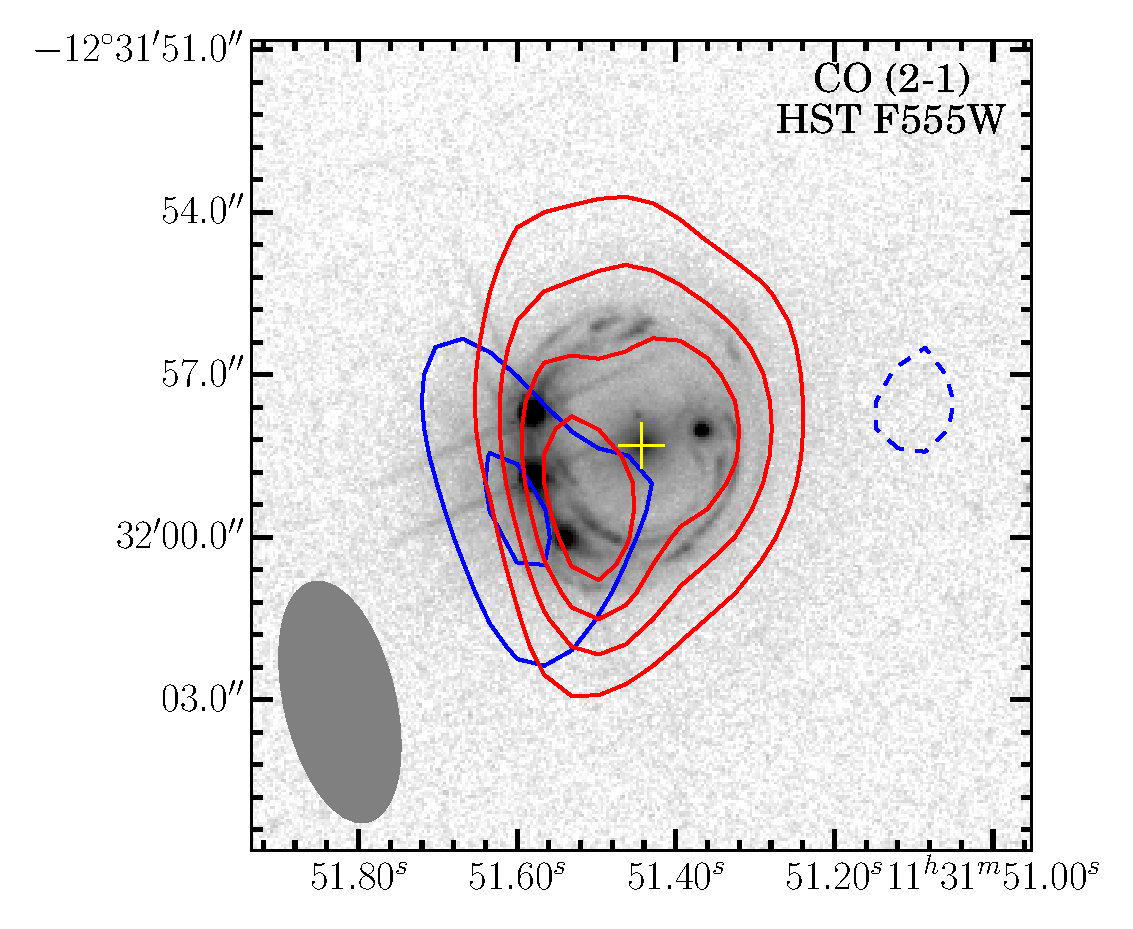
\includegraphics[trim=5 -10 0 0, clip, width=0.472\textwidth]{../Figures/F555W_REDBLUE.eps} 
\\
\includegraphics[trim=25 16 0 10, clip, width=0.85\textwidth]{../Figures/CO_highOmom_CLIP5sigma}
\vspace{0.1em}
\caption{Top left: overlay of the velocity-integrated \bco emission on the archival {\it HST} $V$-band (F555W)
image. 
Top right: same as top left, except the contours are color-coded to represent the red- and blueshifted emission.
The contours in both top panels start at 3$\sigma$ and increment at steps of
$\pm$3$\sigma$, where $\sigma$\,=\,0.3 mJy beam\pmOne for the top left panel, 
and 
$\sigma$ = 0.4 mJy beam\pmOne (red) and 0.5 mJy beam\pmOne (blue)
for the top right panel.
The crosses denote the
location of the foreground galaxy at $z$\,=\,0.295.
Contours for the first (bottom left) and second (bottom right) moment maps of the \bco line emission
are shown in steps of
50 \kms, and 100 \kms, respectively. 
The synthesis beam size is 4\farcs4 $\times$ 2\farcs0, at PA = 13$\degr$.
\label{fig:CO21mom}}
\end{figure*}

We also place an upper limit on \rot[HNC]{2}{1} line emission
in the foreground galaxy at $z\sim$0.295.
Assuming a typical line width of 300\,\kms, this corresponds to a 3$\sigma$
limit of 0.35\,Jy\,\kms\,beam\pmOne.

\subsection{\cco Emission}
We detect \cco line emission toward RXJ1131 at {\bf BLAH}$\sigma$ significance.
The spectrum is shown in \Fig{co32spec}, which appears to be consistent with a 
double-peaked profile. We estimate a line intensity of
35.7\,$\pm$\,21.9{\bf BLAH} Jy\,\kms by summing up fluxes over the FWZI
linewidth used to infer the \bco line intensity ($\sim$700 \kms).
Assuming the spatial extent between \bco and \cco are similar and therefore
magnified by the same amount, the line intensities
correspond to a brightness temperature ratio of
$r_{\rm 32}$\,=\,$T_{\small \cco}$$/$$T_{\small \bco}$\,=\,0.66\,$\pm$\,0.41.

\begin{figure}[!htbp]
%\centering
\includegraphics[width=0.455\textwidth]{../Figures/coOverlay.eps}
\caption{CARMA \cco line profile (solid) without continuum subtraction is
over-plotted on the continuum-subtracted PdBI \bco line profile (dashed).
The velocity scale is with respect to $z$=0.6537, which corresponds to the
dynamical center of the \bco line. The spectral resolution for \cco and \bco
is 35.8 \kms and 21.5 \kms, respectively.
 \label{fig:co32spec}}
\end{figure}



\subsection{Continuum Emission} %DONE
No 1.5\,mm continuum emission is detected at the position of \cco
down to a 3$\sigma$ limit of 2.49\,mJy beam\pmOne.
This is consistent with the spectrum shown in \Fig{co32spec}.

We detect PdBI 2\,mm continuum in \Fig{cont}. The integrated flux density is
1.2\pmm0.2 mJy, with a peak flux
$S_\nu$\,=\,800\pmm88\,$\mu$Jy\,beam\pmOne
centered on the lensing galaxy. Slightly extended emission is also detected
along the lensed arc. This suggests that the detected emission comes from
both the foreground galaxy and the background galaxy and that the
emission is marginally resolved along its major axis.
We subtract a point source model in $uv$-plane to remove the unresolved
emission toward the foreground galaxy. The peak flux (0.39\,$\pm$\,0.08\,mJy)
in the residual map coincides with the lensed arc, and is consistent with
the difference between the integrated and the peak flux in the
original continuum map ($\sim$0.4 mJy). We therefore adopt
$S_\nu$ = 0.39\pmm0.08 mJy as the 2\,mm continuum emission toward
the background galaxy.

\begin{figure}[!htbp]
%\centering
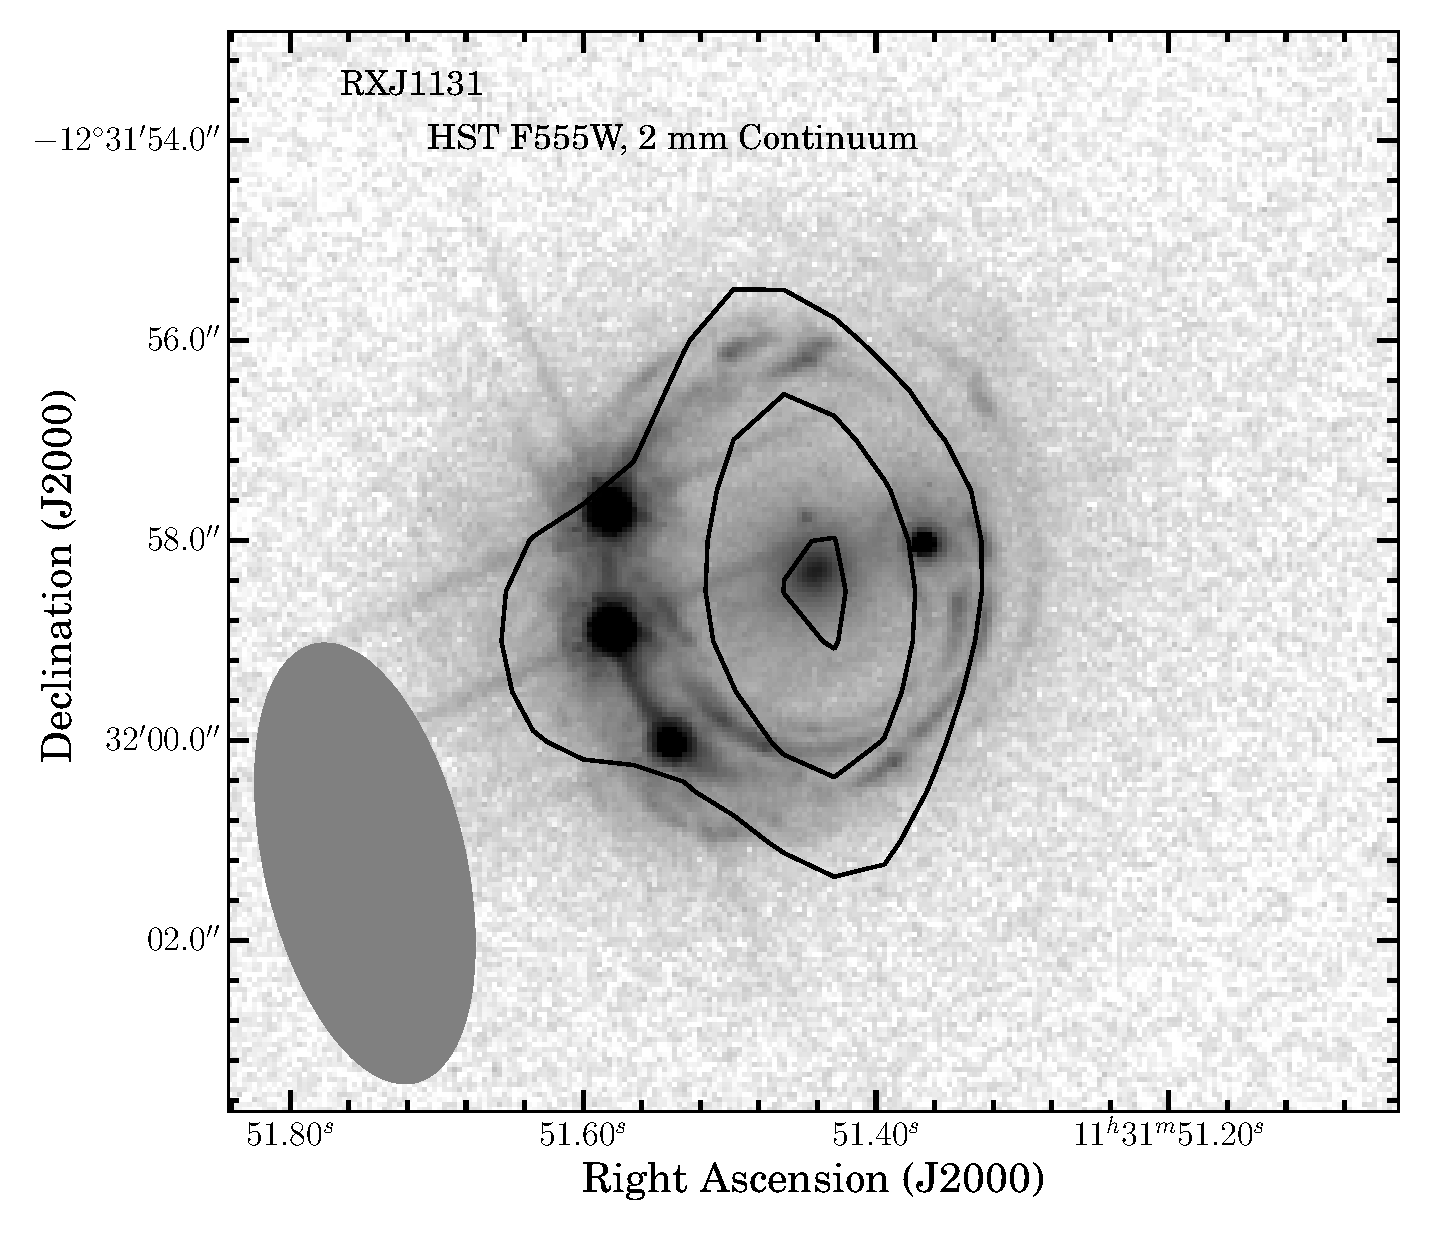
\includegraphics[trim=12 27 0 1, clip, width=0.475\textwidth]{../Figures/F555W_ContPdBI.eps}
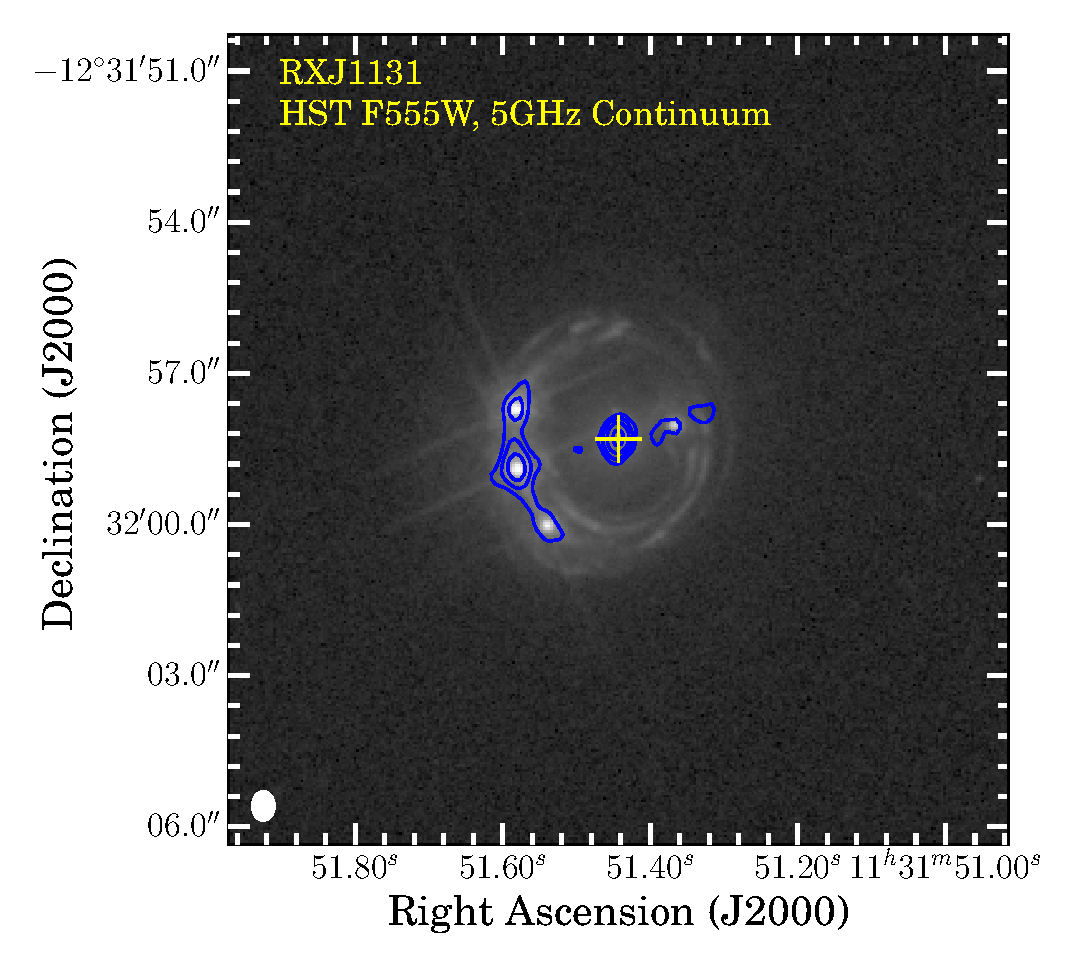
\includegraphics[trim=10 5 0 0, clip, width=0.4695\textwidth]{../Figures/F555W_ContVLA.eps}
\caption{Top: overlay of the 2\,mm continuum emission on the optical image.
Bottom: overlap of the VLA 5\,GHz continuum emission on the optical image.
Contours in both images start and increment at steps of
$\pm$3$\sigma$, where $\sigma_{\rm 2mm}$\,=\,0.082 mJy beam\pmOne and
$\sigma_{\rm 5GHz}$\,=\,13 $\mu$Jy beam\pmOne in the top and bottom panel, respectively.
The central crosses indicate the centroid of the foreground galaxy,
as detected in the optical image. 
The synthesis beam size is 4\farcs4 $\times$ 2\farcs0, at PA = 13$\degr$ for
the PdBI observations (top), and 
0\farcs5 $\times$ 0\farcs4 (PA = 0.18$\degr$) for
the VLA observations (bottom).
\label{fig:cont}}\vspace{0.51em}
\end{figure}

The VLA C-band continuum image in \Fig{cont} shows resolved emission from the
jets and core of the foreground elliptical galaxy
as well as emission toward the background quasar.
Multiple peaks are seen along the arc with their centroids
coincident with the optical emission from the quasar.
We extract the flux densities for the lensing arc and the radio core in \Tab{photometry}.
We find a spectral index of $\alpha^{\rm 2mm}_{\rm 6cm}$\,=\,$-$0.024
for the foreground
galaxy and $\alpha^{\rm 2mm}_{\rm 6cm}$\,=\,$-$0.345
for the background galaxy by fitting a
power-law (S$_\nu \propto \nu^{\alpha}$) to the continuum emission at
5\,GHz and 2\,mm.

\subsection{Photometry} \label{sec:photometry} %DONE
We compile \mir (MIR) to \fir broadband photometry from various
catalogs available on the NASA/IPAC Infrared Science
Archive (IRSA) in \Tab{photometry} with aperture corrections
when warranted. These data were obtained using
the Two Micron All Sky Survey Telescopes \citep[2MASS;][]{Skrutskie06a},
the Wide-field Infrared Survey Explorer \citep[{\it WISE};][]{Wright10a},
the {\it Infrared Astronomical Satellite}
\citep[{\it IRAS};][]{Neugebauer84a}, and
the Multiband Imaging Photometer \citep[MIPS;][]{Rieke04a} and
Mid-infrared Infrared Array Camera \citep[IRAC;][]{Fazio04a} on
the \spitzer.
We retrieve PBCD (level 2) {\it Spitzer}/IRAC images from the
Spitzer Heritage Archive and perform aperture photometry on
the channel 1 image to extract the flux density at 3.6\,$\mu$m
since it is not available from the IRSA archive.

The emission in the IRAC images is slightly extended. We thus use the
{\it HST} image ($\sim$0\farcs07 resolution) to determine
origins of their centroids, all of which are found to be
centered at the position corresponding to the lensed emission from the
background galaxy. To recover the diffuse background emission, we subtract a
point source model centered on the lensing galaxy, using the average
FWHM found by fitting a Gaussian profile to several field stars
with the \ncode{imexam} routine of IRAF.
We perform aperture photometry on the residual image
to obtain decomposed flux measurements from the background galaxy.
The photometry for the foreground galaxy is then obtained
by subtracting the background emission from the
observed total flux. The resulting photometry in
\Tab{photometry} are obtained after performing an aperture correction
described in the IRAC Instrument Handbook\footnote{http://irsa.ipac.caltech.edu/data/SPITZER/docs/irac/iracinstrumenthandbook/} to
correct for the fact that the imaging was calibrated
using a 12$^{\prime\prime}$ aperture, which is larger than the aperture (5\farcs8) we used to
perform aperture photometry.

We fit a power-law spectrum to the
decomposed IRAC photometry to disentangle the background and foreground 
emission from the total flux observed in the MIPS 24\,$\micron$ band. 
The spectral indices corresponding to best-fitting curves are $\alpha$\,=\,$-1.8$ and
$\alpha$\,=\,$-0.85$ for the lensing galaxy and RXJ1131, respectively.
The latter
 is consistent with the mean 3.6\,$-$\,8\,$\micron$
spectral slope of
$\alpha$\,=\,$-$1.07\,$\pm$\,0.53 found for unobscured AGN
\citep{Stern05a}. An extrapolation of the fit to 24\,$\micron$
yields 33.96\,$\pm$\,0.01\,mJy and 25.19\,$\pm$\,0.03\,mJy
for the foreground galaxy and RXJ1131, respectively.
The uncertainties are the standard deviations of 
the extrapolated fluxes obtained from two independent Monte Carlo 
simulations, each of 500 iterations.
% We note that the IRAC photometry includes
% emission from old stellar populations and is prone to
% dust extinction. Hence, the decomposed fluxes are only
% our best estimate of the warm dust emission.
We incorporate the decomposed 24\,$\micron$ data in our
SED fitting to provide some constraints on
the Wien tail beyond the dust peak
of the spectral energy distribution (SED) of RXJ1131.
Details of the SED modeling are presented in \Sec{SED}.

Extraction of the {\it Herschel}/SPIRE photometry at 250, 350, and 500\,$\micron$ was
carried out using \ncode{sussextractor} within the Herschel Interactive
Processing Environment \citep[HIPE;][]{Ott10a}
on Level 2 maps obtained from the Herschel Science Archive.
These maps were processed by the SPIRE pipeline
version 13.0 within HIPE. The \ncode{sussextractor} task estimates
the flux density from an image convolved with a kernel
derived from the SPIRE beam. The flux density
measured by \ncode{sussextractor} is additionally confirmed
using the Timeline Fitter, which performs photometry
by fitting a 2D elliptical Gaussian to the Level 1 data at the
source position given by the output of \ncode{sussextractor}. The fluxes
obtained from both methods are consistent within the uncertainties.

\begin{deluxetable}{lccc}[tbpH]
\tabletypesize{\scriptsize}
\tablecolumns{4}
\tablecaption{Photometry data}
\tablehead{\colhead{Wavelength } & \colhead{Frequency } & \colhead{Flux Density } & \colhead{Instrument}\\ \colhead{micron} & \colhead{GHz} & \colhead{mJy} & \colhead{ }}
\startdata
0.555 & 540167.0 & 0.056 $\pm$ 0.006 & HST-ACS/V-Band(L) \\
0.555 & 540167.0 & 0.009 $\pm$ 0.0041 & HST-ACS/V-Band(H) \\
0.814 & 368295.0 & 0.238 $\pm$ 0.013 & HST-ACS/I-Band(L) \\
0.814 & 368295.0 & 0.041 $\pm$ 0.0054 & HST-ACS/I-Band(H) \\
1.25 & 239834.0 & 1.009 $\pm$ 0.09 & 2MASS/J-Band \\
1.6 & 187370.0 & 0.539 $\pm$ 0.041 & HST-NICMOS(NIC2)/H-Band(L) \\
1.6 & 187370.0 & 0.133 $\pm$ 0.004 & HST-NICMOS(NIC2)/H-Band(H) \\
1.65 & 181692.0 & 1.448 $\pm$ 0.12 & 2MASS/H-Band \\
2.17 & 138153.0 & 2.064 $\pm$ 0.16 & 2MASS/Ks-Band \\
3.4 & 88174.2 & 7.027 $\pm$ 0.14 & WISE/W1 \\
3.6 & 83275.7 & 5.618 $\pm$ 0.0021 & Spitzer/IRAC(Extracted) \\
3.6 & 83275.7 & 5.034 $\pm$ 0.0021 & Spitzer/IRAC(Host) \\
3.6 & 83275.7 & 0.585 $\pm$ 0.003 & Spitzer/IRAC(Archive-Host) \\
4.5 & 66620.5 & 7.803 $\pm$ 0.0021 & Spitzer/IRAC(Archive) \\
4.5 & 66620.5 & 6.009 $\pm$ 0.0017 & Spitzer/IRAC(Host) \\
4.5 & 66620.5 & 1.794 $\pm$ 0.0027 & Spitzer/IRAC(Archive-Host) \\
4.6 & 65172.3 & 8.872 $\pm$ 0.16 & WISE/W2 \\
5.8 & 51688.4 & 10.720 $\pm$ 0.0051 & Spitzer/IRAC(Archive) \\
5.8 & 51688.4 & 7.557 $\pm$ 0.003 & Spitzer/IRAC(Host) \\
5.8 & 51688.4 & 3.163 $\pm$ 0.0059 & Spitzer/IRAC(Archive-Host) \\
8.0 & 37474.1 & 14.470 $\pm$ 0.0041 & Spitzer/IRAC(Archive) \\
8.0 & 37474.1 & 9.881 $\pm$ 0.0039 & Spitzer/IRAC(Host) \\
8.0 & 37474.1 & 4.589 $\pm$ 0.0057 & Spitzer/IRAC(Archive-Host) \\
12.0 & 24982.7 & 21.960 $\pm$ 0.42 & WISE/W3 \\
12.0 & 24982.7 & 400.000 $\pm$ \nodata & IRAS \\
22.0 & 13626.9 & 55.110 $\pm$ 1.9 & WISE/W4 \\
24.0 & 12491.4 & 47.180 $\pm$ 0.026 & Spitzer/MIPS \\
25.0 & 11991.7 & 500.000 $\pm$ \nodata & IRAS \\
60.0 & 4996.54 & 600.000 $\pm$ \nodata & IRAS \\
100.0 & 2997.92 & 1000.000 $\pm$ \nodata & IRAS \\
250.0 & 1199.17 & 289.427 $\pm$ 9.6 & Herschel/SPIRE \\
350.0 & 856.55 & 168.229 $\pm$ 8.6 & Herschel/SPIRE \\
500.0 & 599.585 & 56.782 $\pm$ 8.8 & Herschel/SPIRE \\
1387.93 & 216.0 & 2.492 $\pm$ \nodata & CARMA \\
2152.82 & 139.256 & 1.230 $\pm$ 0.22 & PdBI-integrated \\
2152.82 & 139.256 & 0.799 $\pm$ 0.082 & PdBI-peak \\
2152.82 & 139.256 & 0.400 $\pm$ 0.082 & PdBI-removedFG \\
61414.0 & 4.8815 & 1.273 $\pm$ 0.042 & VLA/Cband-arc \\
61414.0 & 4.8815 & 0.866 $\pm$ 0.027 & VLA/Cband-core
\enddata
\label{tab:BLAH}
\tablecomments{blah}
 %TablenotegoesBetween 
\tablerefs{blah}
\end{deluxetable}


%--------------------------------------------------------------------------
%                                Analysis
%--------------------------------------------------------------------------
\section{Analysis} \label{sec:anal}
%\subsection{Stellar Mass and BH-Bulge Mass Correlation}
%Rest-frame $K$-band (NIR) photometry has been proposed as a reliable proxy to
%the underlying total stellar mass. Using the decomposed IRAC photometry at 3.6$\micron$ (rest-frame $K$-band),
%we find a stellar mass of BLAH, using the BLAH.
%This implies a $M_{\rm BH}$$/$$M^*$ = BLAH (cf. $\sim$0.1\% found in local galaxies).
%
%The AGN-starburst connection has become a central issue with the discovery of the relation
%between stellar velocity dispersion and mass of the central black hole in spheroidal stellar
%systems (Magorrian et al. 1998, Ferrarese & Merritt 2000, Gebhardt et al. 2000). Given that
%elliptical galaxies are mainly old, this relation has to be put in place at their formation history.
%
%This implies that RXJ1131 is in the BLAH stage of the evolution, in which the BH ?.

\subsection{Lens Modeling} \label{sec:lensmodel}
At the angular resolution of the \bco data, the images are resolved over
$\sim$2 resolution elements. 
Given the extent of the lensed emission (see \Fig{CO21mom}),
this implies that we do not resolve
structures (e.g. knots and arcs) of the lensed emission
in our \bco data.
 Nevertheless, the high spectral
resolution of these data provides dynamical information on
spatial scales smaller than the beam (see \Fig{CO21mom}).
Hence, we reconstruct the intrinsic gas dynamics  % - morphology of different kinematic components - velocity structure
by carrying out a parametric lens modeling over different
channel slices of the interferometric data using our lensing code
\uvmcmcfit
(\citealt{uvmcmcfit15a}; see \citealt{Bussmann15a} for details of the code).
Models of each slice thus provide information on 
the corresponding kinematic component of the CO gas, 
enabling us to reconstruct the source plane velocity gradient. 
In order to have adequate SNRs for lens modeling, we bin the frequency channels by a factor of five 
to produce seven independent $\Delta v$\,$\sim$\,105\,\kms channels (dashed line in \Fig{delensed})
that cover the full linewidth of $\sim$750\,\kms. 

\begin{figure}[!htbp]
\centering
\includegraphics[width=0.45\textwidth]{../Figures/de-lensedSpecCO21_complicated_unbinned_ylog.eps}
\caption{The full resolution \bco spectrum (yellow histogram) and 
the binned spectrum (dashed line) with the seven $\Delta v$\,$\sim$\,105\,\kms channels used for lens modeling. The 
blue histogram shows the ``intrinsic'' line profile of RXJ1131 
after subtracting a contribution from its companion galaxy and 
correcting for lensing using the magnification factors $\mu_{\rm L}$ as annotated with horizontal bars
above the respective model channels. Flux density is shown on a log scale along the y-axis.
\label{fig:delensed}}
\end{figure}

The lens mass distribution is modeled using a singular isothermal
ellipsoid (SIE) profile, which is described by five free parameters: the
positional offset in R.A. and Dec. relative to an arbitrary chosen
fixed coordinate in the image, the Einstein radius, the axial ratio, and the
position angle. We use the VLA radio continuum emission toward
the foreground galaxy to initialize the positional offset. We impose a
uniform prior $\pm$0\farcs05 in both $\Delta$R.A. and $\Delta$Dec.,
motivated by the astrometry uncertainties in the VLA image as well as
the uncertainties provided by previous SIE lens model \citepalias{Claeskens06a}.
We initialize the Einstein radius based on the model parameters reported by \citetalias{Claeskens06a}
and impose a uniform prior using $\pm$3$\sigma$ of their uncertainties.
The sources are modeled using elliptical Gaussian profiles, which are
parameterized by six free parameters: the positional offset in R.A.
and Dec. relative to the lens, the intrinsic flux density, the effective
radius, the axial ratio, and the position angle. The position of each source
is allowed to vary between $\pm$1\farcs5 (i.e., within the Einstein radius)
and the effective radius is allowed to vary from 0\farcs01$-$2$^{\prime\prime}$.

Our code uses an Markov Chain Monte Carlo (MCMC) approach to sample the
posterior probability distribution function (PDF).
In each model, we require a target acceptance rate of $\sim$0.25$-$0.5
and check for chain convergence by inspecting trace plots
and requiring the samples are beyond at least an autocorrelation time.
We thus employ $\sim$50,000 samples as the initial ``burn-in'' phase
to stabilize the Markov chains (which we then discard) and
use the final $\sim$5,000 steps, sampled by 128 walkers, to identify
the posterior. Here, we
identify the best-fit model and the quoted uncertainties using the
median and the 68\% confidence intervals in the marginal PDFs.
\begin{deluxetable*}{lcc}[!htbp]
\tabletypesize{\scriptsize}
\tablecolumns{3}
\tablecaption{Lens parameters from preliminary models}
\tablehead{
\multicolumn{2}{c}{Parameters} &
\colhead{Median values} % weighted-mean of median of each
}
\startdata
Offset in RA    & (\arcsec)   &  0.004$\pm$0.027\\
Offset in Dec    & (\arcsec)   & 0.003$\pm$0.027\\
Axial Ratio      &             & 0.56$\pm$0.16\\
Position Angle   & (deg)       & 103$\pm$22\\
Einstein Radius  & (\arcsec)   & 1.833$\pm$0.002\\
\enddata
\label{tab:lens}
\tablecomments{ Parameters describing the foreground lens are
obtained based on the preliminary models (see text for details).
All angular offsets are with respect to
$\alpha$\,=\,11$^{\rm h}$31$^{\rm m}$51\fs44,
$\delta$\,=\,-12\degr31\arcmin58\farcs3 (J2000).
The corresponding masses
within the Einstein radii is $M(\theta$\,\,$<$\,\,$\theta_\textrm{E})$\,=\,(7.47\,$\pm$\,0.02)\,$\times$\,10$^{11}$\,\,\Msun.}
\end{deluxetable*}


We first obtain a preliminary lens model for each channel slice independently,
where their lens parameters are allowed to vary and are initialized according
to the aforementioned way. We obtain the final model
by repeating the modeling over each slice but fixing their lens parameters
to the overall median in the preliminary models,
as listed in \Tab{lens}.
This ensures that all models share the same lens profile.
The magnification factors in \Tab{model} are determined by taking the ratio
between the image plane flux and the source plane flux of each model.

Our model parameters in \Tab{lens}, describing
the mass distribution of the lensing galaxy, are consistent (within the uncertainties)
with that of the SIE model presented by \citetalias{Claeskens06a}. We find a mass of
$M(\theta$\,\,$<$\,\,$\theta_\textrm{E})$\,=\,(7.47\,$\pm$\,0.02)\,$\times$\,10$^{11}$\,\Msun
within the Einstein radius.

\subsubsection{Interpretation of the Source-plane Morphology} \label{sec:caveat}
The reconstructed source locations in \Fig{model} demonstrate
an intrinsic velocity gradient across the source plane, which is
consistent with a kinematically-ordered disk-like galaxy.
Additional support to the disk conjecture
can be found in the double-horned line profile (\Fig{CO21spec})
and the observed (image plane) velocity field (\Fig{CO21mom}). Furthermore,
\citetalias{Claeskens06a} also find that the reconstructed source plane emission in optical-NIR
is best-reproduced using a $n$\,=\,1 Sersic profile.
We thus interpret RXJ1131 as a disk galaxy.

% the companion
A better fit is found for the lens model of
the red-most channel if we add a second source component (see
top left panel in \Fig{model}). This is consistent with previous results
reported by \citet[hereafter B08]{Brewer08a}, who find an optically faint companion
(component F in their paper) $\sim$2.4\,kpc in projection from the AGN host galaxy in $V$-band,
and with \citetalias{Claeskens06a}, who find evidence for an interacting galaxy near RXJ1131.
Spatially, the red velocity component of the CO emission
also coincides with this component F. It is therefore likely that we
detect \bco emission in a companion galaxy.
\defcitealias{Brewer08a}{B08}

The type of merger (major v.s. minor) in a pair of interacting galaxies 
is most commonly distinguished based on 
the ratio between their total galaxy mass.
Here, we use the gas mass ratio between RXJ1131 and
its companion galaxy instead, given that we do not have constraints on their individual galaxy mass.
We decompose the total line flux into two components:
one from RXJ1131 and the other from its companion.
Since the companion is only detected in the red-most channel, we
derive its intrinsic gas mass using the best-fit flux 
densities and magnification factors obtained from the models of this channel.
Assuming a brightness temperature ratio 
of $r_{\rm 21}$\,=\,1 between \bco and \aco lines and
a CO luminosity-to-H$_2$ mass conversion factor of
\alphaco\,=\,0.8\,\alphaU, we find
a molecular gas mass of $M_{\rm gas}$\,=\,$($1.92\pmm0.09$)$\,\E{9} \Msun.
%statistical unc. only (i.e. draw from distributions of on mag. factor & intrinsic flux)
For the molecular gas mass in RXJ1131, we derive
its intrinsic line flux over the FWZI linewidth
using the respective magnification
factors listed in \Tab{model}, which to
first order takes into account effect of differential lensing.
This yields $I_{\small \bco}$\,=\,2.93\pmm0.70 Jy\,\kms,
where the uncertainty includes those on
the magnification factors.
Adopting the same brightness temperature ratio and \alphaco\ as
used for the companion, this corresponds to a gas mass of
$M_{\rm gas}$\,=\,$($1.38\pmm0.33$)$\,\E{10} \Msun, which
implies a {\em gas} mass ratio of $\sim$7:1 between RXJ1131 and its companion.
We thus classify the system to be a {\em ``wet-wet'' minor merger}.
We caution that this is based on their gas mass ratio rather than their total galaxy mass ratio, which 
is more commonly used in literature as the
classification scheme to separate major mergers from minor mergers. 

The spatial resolution of the data in hand
is a few arcsec, which implies that despite the high SNR and spectral
resolution, constraints on the intrinsic sizes of the lensed galaxies are modest, and thus the magnification
factors may be under-predicted. % see Bussmann15

\begin{figure*}[tbph]
\centering
\begin{tabular}{c}
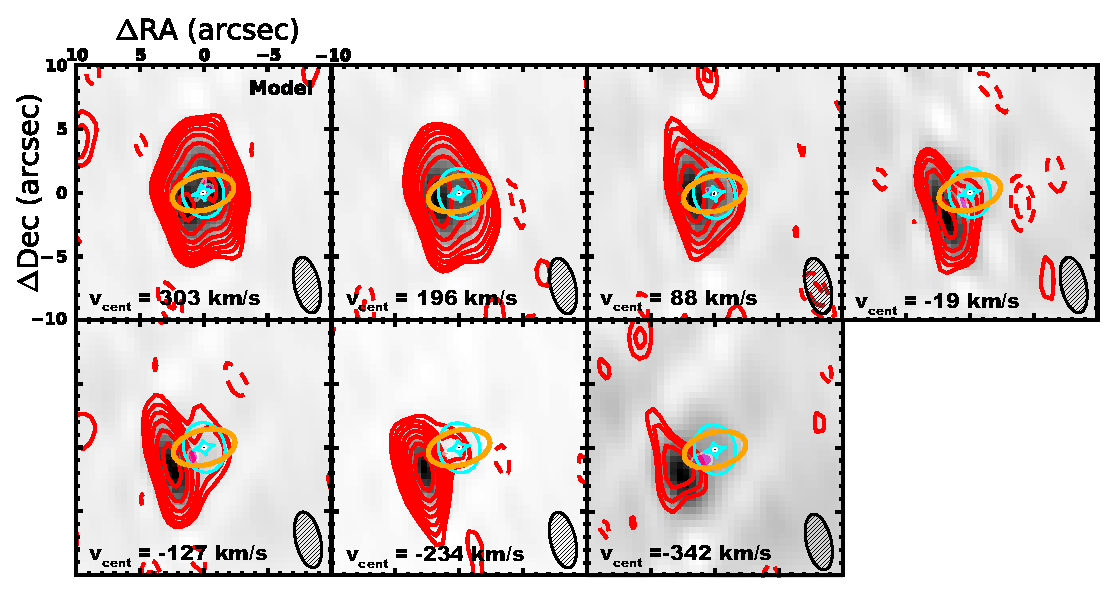
\includegraphics[trim=0 0 0 0, clip, width=1.0\textwidth]{../Figures/PostageStampModel.eps} \\
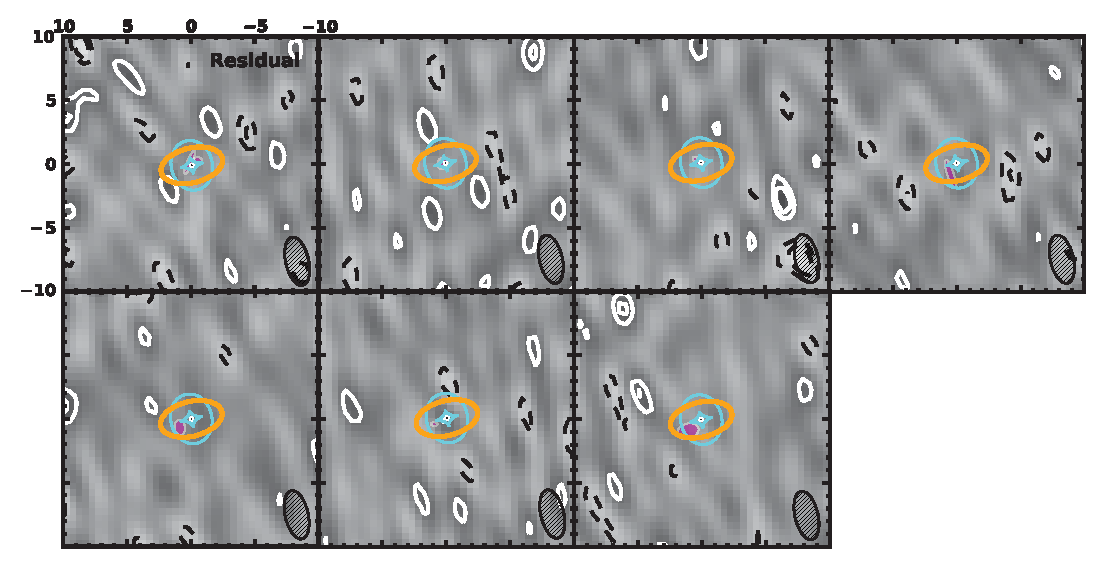
\includegraphics[width=0.98\textwidth]{../Figures/PostageStampResiduals.eps}
\end{tabular}
\caption{Each panel corresponds to a lens model of RXJ1131 performed over a
channel slice $\sim$100\,\kms of the \bco data. Top: channel maps of the
PdBI \bco emission (red) overlaid on our best-fit lens models (grayscale).
The location of the foreground lensing galaxy is indicated by a black dot and
its critical curve is traced by the orange solid line. The locations and
morphologies (half-light radii) of the reconstructed sources are
represented by magenta ellipses.
The caustic curves are represented as cyan lines. The beam of the
PdBI observations is shown in the bottom right corner of each panel.
Bottom: residual images of the best-fit models, obtained by
taking the Fourier transform after subtracting the best-fit model from the
data in the $uv$-domain. Contours start
at $\pm$3$\sigma$ and increment at steps of 3$\times$2$^n\sigma$,
where $n$ is a positive integer.
\label{fig:model}}
\end{figure*}

\subsubsection{Spatial Extent and Differential Lensing} \label{sec:differential}
In the image plane shown in  \Fig{CO21mom}, the redshifted component is
cospatial with the Einstein ring seen in the
optical image, with most of its apparent flux originating from the lensed arc
in the southeast, whereas the blue component is predominately coming from
solely the lensed arc. To further illustrate this, we show the
channel maps of 21.5\,\kms width and a spatial spectra map of 1\farcs5 resolution in
\Fig{chanmap} and \Fig{spatialSpec}, respectively. The figures
show that emission
is present to the west, peaking toward the lensing arc (black crosses in
\Fig{chanmap}) in the red wing, and shifts to the east with decreasing velocity
(blue wing).
This is consistent with the source plane positions in our models and
is suggestive of an extended CO emitting region.

\begin{figure*}[!htbp]
\centering
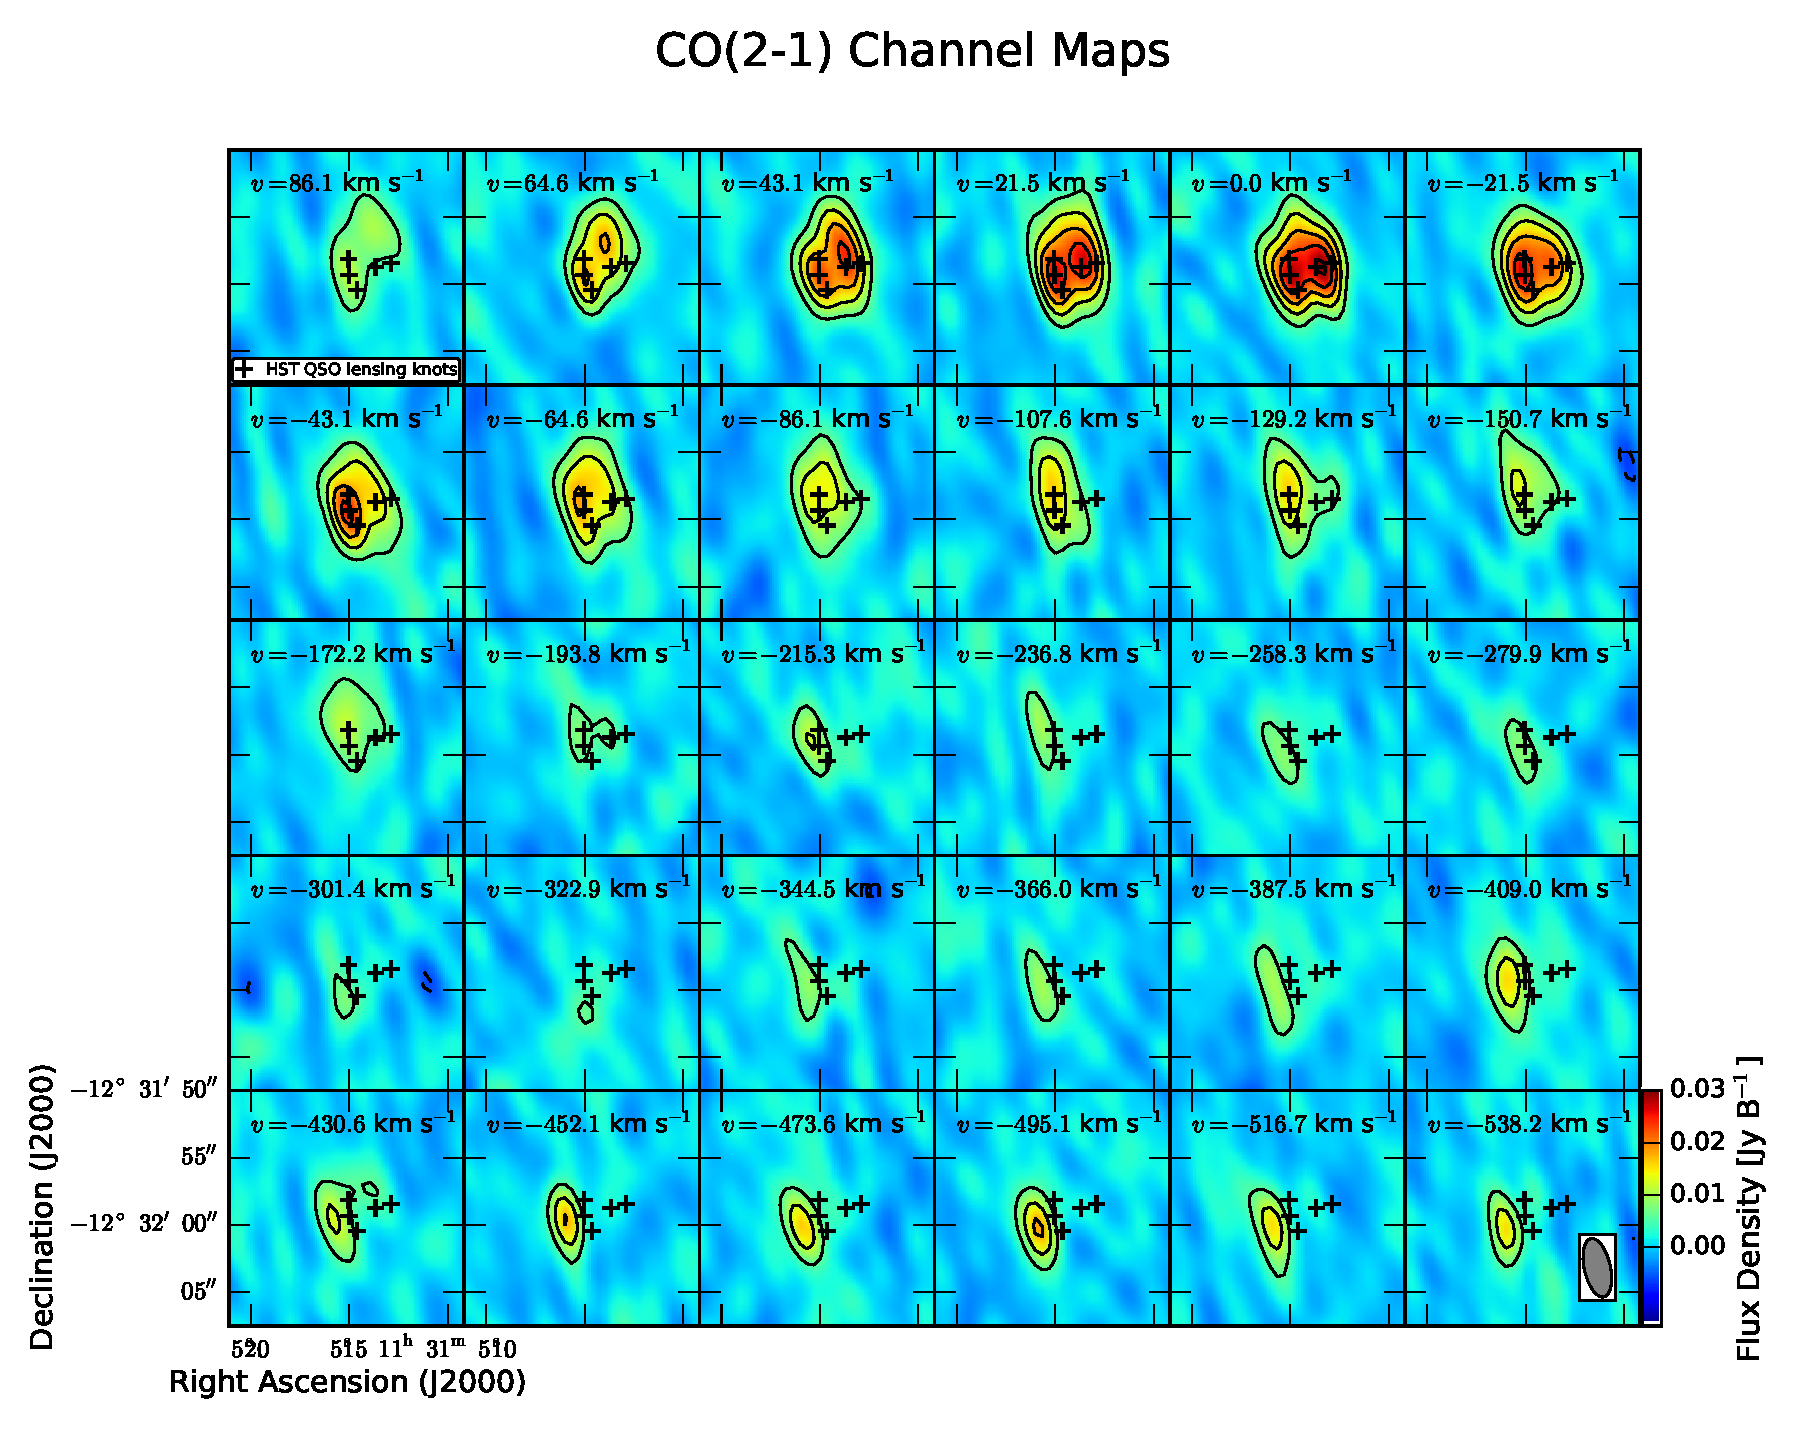
\includegraphics[width=1.0\textwidth]{../Figures/co_channel_maps.eps}
\caption{
Channel maps of the PdBI \bco data cube toward RXJ1131 at 21.5\,\kms resolution.
Black crosses indicate the positions of the lensed knots (AGN emission,
which correspond to components ABCD in \citetalias{Claeskens06a}). The central white-filled
star indicates the position of the foreground lensing galaxy (component G
in \citetalias{Claeskens06a}).
Central velocities are shown at the top of each map.
Contours start and increment at steps of
$\pm$3$\sigma$. The beam is denoted in the bottom right panel. \label{fig:chanmap}}
\end{figure*}

\begin{figure*}[!htbp]
\centering
\includegraphics[width=0.9\textwidth]{../Figures/spatialSpec_offsetShifted.eps}
\caption{
\bco spectrum as a function of position, binned by 3 pixels in each
direction (1\farcs5).
The spectra map covers an extent of $\sim$10"$\times$10"
centered on the pixel that corresponds to the lensing galaxy.
Spatial offset in arcsec is denoted in top left corner of each panel.
The velocity and flux density scales are denoted in the top right panel.
\label{fig:spatialSpec}}
\end{figure*}

\begin{deluxetable}{lcc}[!htbp]
\tabletypesize{\scriptsize}
\tablecolumns{3}
\tablecaption{Magnification factors of various kinematic components in \bco}
\tablehead{
\colhead{Velocity Range(\kms)} & % see 22May16/intensity30Apr16.spec; or channel map in paper
\colhead{Source 1 $\mu_{\rm L}$} &
\colhead{Source 2 $\mu_{\rm L}$}
}
\startdata
$-$366\,$-$\,$-$258 & 3.1 $\pm$ 0.9 & \\ [0.5ex]
$-$237\,$-$\,$-$151 & 4.3 $\pm$ 2.4 & \\ [0.5ex]
$-$129\,$-$\,$-$43  & 4.2 $\pm$ 0.6 & \\ [0.5ex]
$-$21.5\,$-$\,65    & 4.1 $\pm$ 0.9 & \\ [0.5ex]
86\,$-$\,172        & 8.7 $\pm$ 2.0 & \\ [0.5ex]
194\,$-$\,280       & 7.6 $\pm$ 1.6 & \\ [0.5ex]
301\,$-$\,388       & 7.2 $\pm$ 5.6 & 6.7 $\pm$ 2.5 \\ [0.5ex]
weighted average & 4.4 & \\ [0.5ex]
median & 5.5 &
\enddata
\label{tab:model}
\tablecomments{Velocity is taken from the center of each (native) channel
without any binning. Each row corresponds to a channel slice used for
lens modeling. Source 1 is RXJ1131 and source 2 is its companion. See text for details. }
\end{deluxetable}


Similar to previous studies of RXJ1131, where
differential lensing across {\it HST}
$V$-, $I$-, and $H$-band has been detected with a
magnification factor decreasing from 10.9 to 7.8 \citepalias{Claeskens06a},
the highly asymmetric \bco line profile suggests that
differential lensing is also non-negligible for CO,
causing the redshifted emission to be apparently much brighter than the
blueshifted component and the asymmetric line profile.
This can be explained by the difference in magnification factor $(\mu_{\rm L})$ which
varies from 8.7 to 3.1 across the \bco line (\Tab{model}) and also partly due to a contribution from the companion in the redshifted velocity channels.
The variation in $\mu_{\rm L}$ across channels is consistent with the source plane
positions relative to the caustics in \Fig{model}, where the red wing
emission mainly originates near the cusp
of the caustic and the blue wing emission is located beyond the caustics.
In fact, the intrinsic line flux of the redshifted and
blueshifted emission in RXJ1131 (after subtracting a contribution from the companion)
is $I_{\small \bco}$\,=\,1.26\pmm 0.23 Jy\,\kms and 1.25\pmm0.23 Jy\,\kms, respectively,
implying an intrinsically symmetric line profile (\Fig{delensed}). This is consistent with the source-plane
velocity gradient in our lens model (\Fig{model} and \Fig{PV}).
% The difference in magnification factors between CO and optical-to-NIR
% may further indicate that the CO emitting region is more extended and/or
% has a spatial offset from the optical-to-NIR emission
% (\ie different positions and alignment relative to the caustics) given
% the lower magnification factor found for CO (median $\mu_{\rm L}$ = 5.5)
% than in NIR, while their spatial extents appear to be similar. But then it could just be because of the low resolution and
% the degeneracy between the intrinsic source size and the magnification factor.

\subsection{\bco Kinematics}
Fitting a four-parameter double-Gaussian that describes two velocity peaks by a single FWHM
to the ``intrinsic'' \bco line profile of RXJ1131 (after correcting for lensing using
the magnification factors for various channels and separating the emission from RXJ1131 and its companion),
we find a roughly symmetric double-horned profile with a flux ratio of 1.2\pmm0.4 between the peaks, which
are separated by
$\Delta v_{\rm sep}$ = 387\pmm45\,\kms, and a
FWHM of 220\pmm72\,\kms.
The peak separation obtained from this ``intrinsic'' line profile is 
slightly lower than that obtained from the observed spectrum (\ie without lensing corrections).
This discrepancy is likely a result of differential lensing, which causes the line peak of the red wing 
to shift towards higher velocity channels, biasing the centroid of
one of the components in a double-Gaussian to higher velocity than otherwise.
If we instead fit with a single-Gaussian, we find a FWHM of 600\pmm160\,\kms for RXJ1131
and 73\pmm43\,\kms for the companion galaxy.

A clear velocity gradient and a high
velocity dispersion ($\gtrsim$400\,\kms) near the central region
is seen in \Fig{CO21mom}. While beam smearing is inevitably the
dominant factor in the observed velocity dispersion
at the spatial resolution of these data, the exceedingly
high velocity dispersion may hint
at potential perturbations from the AGN, or internal turbulence due to
interactions with the companion, and/or instability due to the large gas
content.
Therefore, in this scenario, RXJ1131 is
consistent with a disrupted disk galaxy hosting an optically
bright quasar and is in the process of merging.

\subsection{\bco Dynamical Modeling} \label{sec:dynamics} 
Assuming the velocities of the respective channels used in the
lens modeling correspond to solely the tangential component of the
true velocity vector of a rotating disk (i.e., along the major axis),
we extract a one dimensional PV diagram in \Fig{PV}
by slicing across their source plane positions (PA: 121\degr).

We then attempt to characterize the molecular gas kinematics using an
empirically-motivated disk model \citep[\eg][]{Courteau97a,Puech08a,Miller11a}:
\begin{equation}
V = V_0 + \frac{2}{\pi} V_{a} \arctan(\frac{R}{R_{t}}),
\end{equation}
where $V$ is the observed velocity, $V_0$ is the velocity at dynamical center,
$V_{a}$ is the asymptotic velocity, and $R_{t}$ is the ``turnover''
radius at which the rotation curve becomes flat.
We perform non-linear least square fitting using an orthogonal distance
regression to find the best-fit parameters,
taking into account the uncertainties in both velocity (channel width) and
distance offset. We also place an upper limit on $R_{t}$\,$<$15 kpc
to keep this parameter physical \citep[\eg][]{Puech08a,Miller11a}.
The parameter uncertainties are inferred based on a Monte Carlo simulation
of 500 iterations, where the input parameters are perturbed
according to random Gaussian distributions of sigmas
corresponding to their uncertainties.
Using this model, we find $V_{a}$\,=\,975\,$\pm$\,387 \kms,
$R_{t}$\,=\,10.7\,$\pm$\,5.7\,kpc, and $V_0$\,=\,28\,$\pm$\,40 \kms.
However, since emission is not resolved along the flat regime
of the rotation curve, the asymptotic velocity is poorly constrained and
the ``turnover'' radius is at most an upper limit.
In particular, $V_{a}$ and $R_{t}$ are highly correlated with a
Pearson coefficient $R$\,=\,0.998, and 0.027 between $V_{a}$ and $V_0$.

\begin{figure*}[!htbp]
\centering
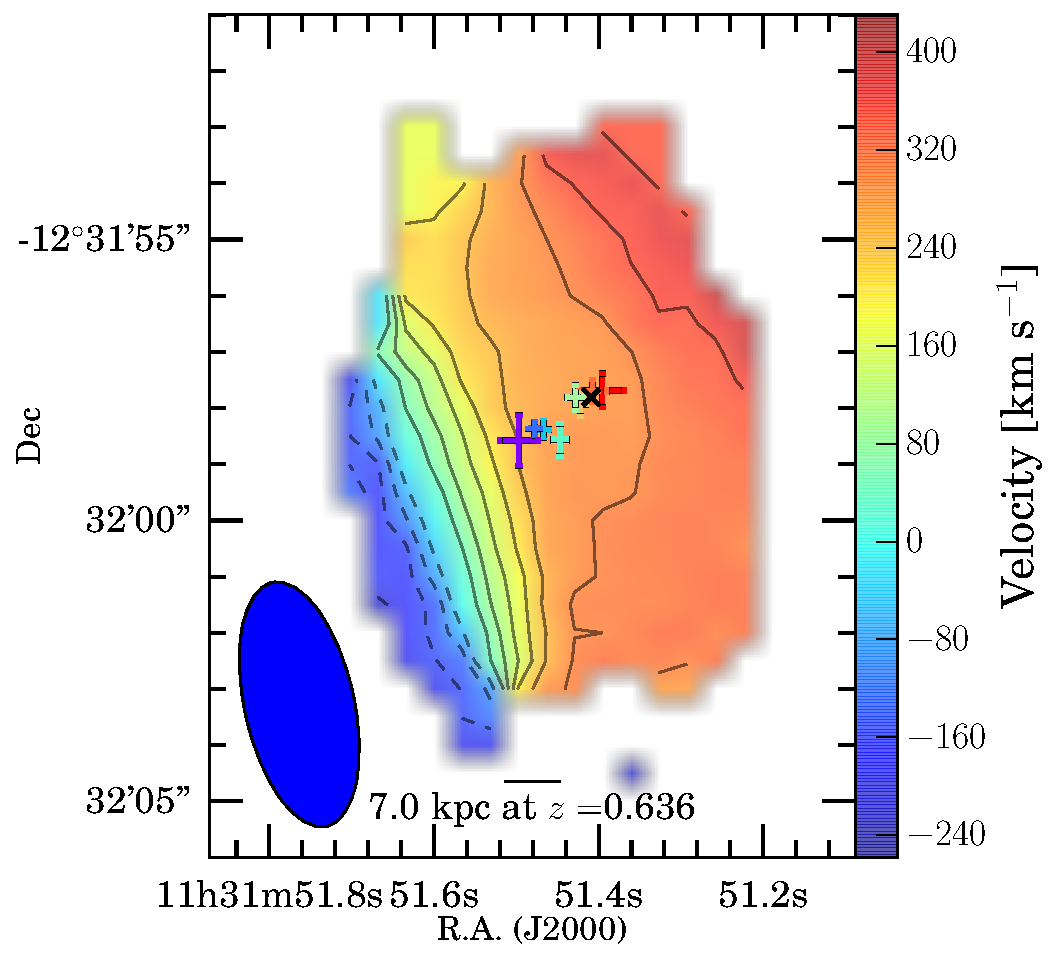
\includegraphics[trim=0 0 30 0, clip, width=0.4\textwidth]{../Figures/veloGradient_markers}
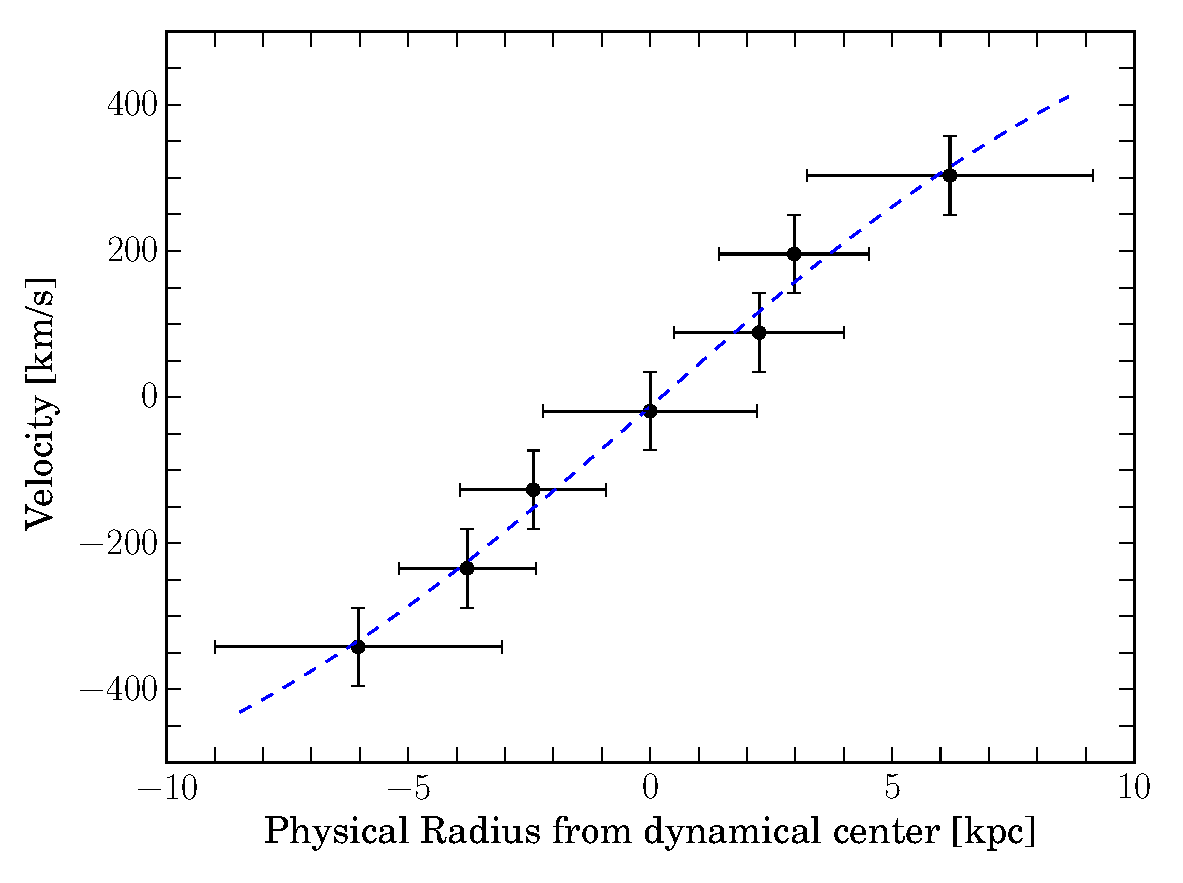
\includegraphics[width=0.525\textwidth]{../Figures/bestfit_PV.eps}
\caption{Left: Source-plane positions from best-fit \bco lens models are indicated with their associated uncertainties atop
the observed first moment map. The contours are at steps of 50\,\kms.
Right: PV slice along the major axis in the source plane at PA\,=\,121\degr.
Dashed line shows the best-fit rotation curve using an arctangent model.
The vertical error bars show the channel width for
each model and the horizontal error bars are the
1$\sigma$ uncertainties on the source plane positions.
 \label{fig:PV}}
\end{figure*}

The asymptotic velocity ($V_{a}$) -- an extrapolation of the model
out to radius beyond the disk scale-length and half-light radius --
is not equivalent to maximum observed velocity ($V_{\rm max}$),
which is commonly used in literature to parameterize disk rotation.
The arctangent model is most commonly used in studies of the
Tully-Fisher relation, where an extrapolation to V$_{2.2}$ (velocity
at 2.2 disk scale-length or $\sim$1.375 half-light radius,
or $\sim$0.7$R_{\rm opt}$\footnote{Radius enclosing 83\% of the light
distribution.}) is typically adopted
as the rotation velocity ($V_{\rm max}$ in their
terminology) since this corresponds to the radius at which the velocity
of a pure exponential disk peaks \citep{Courteau97b}.
We here adopt the maximum {\em observed} velocity
$V_{\rm rot}$\,=\,345\,$\pm$\,55\,\kms at 6\,$\pm$\,3\,kpc from the % line center velo of the reddest channel slice, unc = slice width
dynamical center as a proxy to the rotation velocity.
This radius corresponds to $\sim$0.6$R_e$, where $R_e$ is the half-light
radius $\sim$10.3\,kpc inferred from the {\it HST} $I$-band
lens model (\citetalias{Claeskens06a}; converted to
our cosmology).
We note that the source plane half-light radius varies substantially with
wavelength. In particular, the half-light radius is found to be
$\sim$\,4\,kpc and $\sim$7\,kpc in $V$-band
\citepalias{Brewer08a} and $H$-band \citepalias{Claeskens06a}, respectively.
The CO gas is thus of similar spatial
extent as in $H$ and $I$-bands.

In the rest-frame,
emission in the observed-frame $H$-band corresponds to NIR emission $(\sim$1\,$\micron)$,
tracing radiation from the accretion disk surrounding
the central AGN and also from old and evolved stellar populations;
$I$-band corresponds to roughly the optical $V$-band, tracing stellar radiation from
existing, less massive (\ie longer-lasting) stars;
$V$-band corresponds to roughly $U$-band,  tracing radiation from massive young stars
in the host galaxy. Hence,
the $V$-band compactness may be explained in part
due to the fact that its emission is
more susceptible to dust extinction than in other bands and/or
a central starburst caused by higher
concentrations of star-forming gas towards the central regions -- owing to
gravitational perturbations induced
from interactions with the companion
\citep[\eg][]{DiMatteo05a}.
This is consistent with the picture that old stars form first and constitute the bulge component
of a spiral galaxy and that nuclear starbursts (in the inner few kpc) can be triggered 
in a later time as the progenitor disk galaxy interacts with other galaxies, 
and thereby forming a larger bulge.

\subsection{SED Modeling} \label{sec:SED}  % DONE
We fit dust SED models to the
24\,\micron$-$2.2\,mm photometry in \Fig{SED}, where we also
include the IRAS 60\,$\micron$ and 100\,$\micron$ upper limits
to constrain the dust peak.
The fit is performed with the code
\ncode{mbb\_emcee} \citep[\eg][]{Riechers13a,Dowell14a}, which samples the posterior
distributions using an MCMC approach and uses instrumental
response curves to perform color correction on-the-fly.
The SED model consists of a modified-blackbody
function with a power-law attached to the
Wien side to account for an excess in the MIR owing to emission of
warm and small dust grains.
% Previous studies find that in the absence of mid-IR data, a powerlaw slope
% of $\alpha$ = 2 is consistent with SB and slightly more shallow, $\sim$1.5, % for SB/AGN composite systems (Blain et al., 2003; Casey, 2012; Koss et al., 2013).
%
%We add $\sim$15\% calibration uncertainties in quadrature to obtain the total
%uncertainties for the PdBI continuum in our fitting procedure.
The model is thus described by five free parameters: the rest-frame characteristic dust
temperature ($T_{d}$), the emissivity index ($\beta$), the power-law index
($\alpha$), the flux normalization at 500\,$\micron$ ($f_{\rm norm}$), and
the observed-frame wavelength at which the emission
becomes optically thick ($\lambda_{0}$). We impose
a uniform prior with an upper limit of 100\,K on $T_d$ \citep[see \eg][]{Sajina12a},
a Gaussian prior centered around
$\mu$\,=\,1.9 with $\sigma$\,=\,0.3 on $\beta$, and a uniform prior with an upper limit of
1000\,$\micron$ on $\lambda_0$.
We check for chain convergence by requiring that the autocorrelation
length of each parameter is less than the number of steps
taken for the burn-in phase (which are then discarded).
Here we report the statistical means % modes in log file
% summary statistics (global mode (where min. chi),
% marginal mode (in log file), posterior median (instead of posterior means;
% need to compute)
and the 1$\sigma$ confidence interval in the marginal PDFs
as the best-fit parameters, as listed in \Tab{SED}.

\begin{deluxetable}{lccc}[!htbp]
\tabletypesize{\scriptsize}
\tablecolumns{4}
\tablecaption{SED fitting results}
\tablehead{
\multicolumn{2}{c}{Parameters}      &
\colhead{With 24\micron} &
\colhead{Without 24\micron}
}
\startdata
$T_d$                           & (K)                & 52.0\petm{4.0}{4.1}   & 58.2\petm{14.5}{14.4}  \\ [1.05ex]
$\beta$                         &                    & 1.8\petm{0.5}{0.6}    & 2.1\petm{0.3}{0.3}  \\ [1.05ex]
$\alpha$                        &                    & 1.6\petm{0.5}{0.5}    & 8.9\petm{6.9}{6.3}   \\ [1.05ex]
$\lambda_0$\tna                 & ($\micron$)        & 548\petm{285}{307}    & 367\petm{125}{145}  \\ [1.05ex]
$\lambda_{\rm peak}$\tnb        & ($\micron$)        & 162\petm{16}{30}      & 146\petm{39}{44}  \\ [1.05ex]
$f_{\rm norm,\ 500\micron}$\tnc & (mJy)              & 59\petm{14}{13} & 60\petm{5}{5} \\ [1.05ex]
\LFIR\tnd                       & (10$^{12}$\,\Lsun) & 3.81\petm{2.04}{1.92} & 4.72\petm{2.54}{2.26}      \\ [1.05ex]
$M_{\rm d}$\tne                 & (10$^8$\,\Msun)    & 22\petm{5}{18}        & 11\petm{5}{6}
\enddata
\label{tab:SED}
\tablenotetext{a}{Observed-frame wavelength where $\tau_\nu$\,=\,1}
\tablenotetext{b}{Observed-frame wavelength of the SED peak}
\tablenotetext{c}{Observed-frame flux density at 500 $\micron$}
\tablenotetext{d}{Rest-frame 42.5$-$122.5\,$\micron$ luminosity}
\tablenotetext{e}{Derived assuming absorption mass coefficient of $\kappa$\eq2.64\,m$^2$\,kg$^{-1}$ at $\lambda$\,=\,125.0\,$\micron$ \citep{Dunne03a}}
\tablecomments{Errors reported here are $\pm$1$\sigma$.
\LFIR and $M_{\rm d}$ are not corrected for lensing.}
\end{deluxetable}


In the first model, we include the 24\,$\micron$ data
to constrain the power-law index. Based on the
best-fit of this model, we find an apparent
\fir luminosity (rest-frame 42.5\,$-$\,122.5\,$\micron$) of
3.81\petm{2.04}{1.92}\E{12}\,\Lsun and a
dust mass of 22\petm{5}{18}\E{8}\,\Msun, uncorrected for lensing.
For the mass absorption coefficient, we adopt
$\kappa$\,=\,2.64\,m$^2$kg\pmOne at rest-frame 125.0\,$\micron$
\citep{Dunne03a}.
The dust mass uncertainty does not
include that of the absorption coefficient.

A fit including the MIR 24\,$\micron$ photometry
is likely an upper limit on the \fir luminosity due solely to \SF
in the AGN host galaxy.
% since the fit include contribution from the AGN (through power-law to MIR)
If we instead fit for a model excluding this constraint,
two major consequences are immediately apparent.
First, the power-law index is poorly-constrained (see \Tab{SED}).
Second, the steep power-law implies only a small contribution
from the power-law regime
to the total IR luminosity as compared to the graybody component.
Thus, the \fir luminosity in
this model should, in principle, correspond to a
lower limit on the cold dust emission.
Using the best-fit parameters
for this model, we find a total IR luminosity
\LIR (rest-frame 8\,$-$\,1000\,\micron) of 9.71\petm{6.14}{-6.05}\E{12}\,\Lsun,
a \fir luminosity \LFIR of 4.72\petm{2.54}{2.26}\E{12}\,\Lsun and a
dust mass $M_{\rm dust}$ of 11\petm{5}{6}\E{8}\,\Msun, all of which are uncorrected for lensing.
Taken at face value, this implies a FIR-to-IR luminosity ratio
of $\sim$58\pmm35\%.

The dust temperature from both models is similar to that of
ULIRGs at 0.6\,$<$\,$z$\,$<$\,1.0 (54\,$\pm$\,5\,K;
\citealt[hereafter C13]{Combes13a}).
We note the \fir luminosity is comparable in both models, which is
not surprising given the lack of constraints in the MIR.
For the subsequent analysis, we adopt the physical quantities
from the first model (\ie with constraints at 24\,\micron).
The choice of SED model does not affect
the derived star formation rate (SFR) given the similar \fir luminosity.
Yet, the dust mass is higher by a factor of $\sim$2 in the former but consistent within the
uncertainties.
We correct for lensing using the median magnification
factor $(\mu_{\rm L}\eq5.5)$
from the CO lens models. This yields a
 \LFIR of $($6.9\pmm3.6$)$\E{11}\,\Lsun
 and
 a total IR luminosity of $\sim$1.5\E{12}\,\Lsun,  implying RXJ1131 is a ULIRG.
Assuming a Salpeter initial
mass function \citep{Salpeter55a}, we find a
SFR$_{\rm FIR}$ of 120\pmm63\,\sfrU using a
standard conversion \citep{Kennicutt98a}.
\defcitealias{Combes13a}{C13}

% WISE flux is slightly higher than the IRAC point, probably due to a smaller
% aperture used in IRAC extraction (both from archive).
% It is also not straight-forward to fit an SED model covering a wider wavelengths because of
% differential lensing.
\begin{figure}[!htbp]
\centering
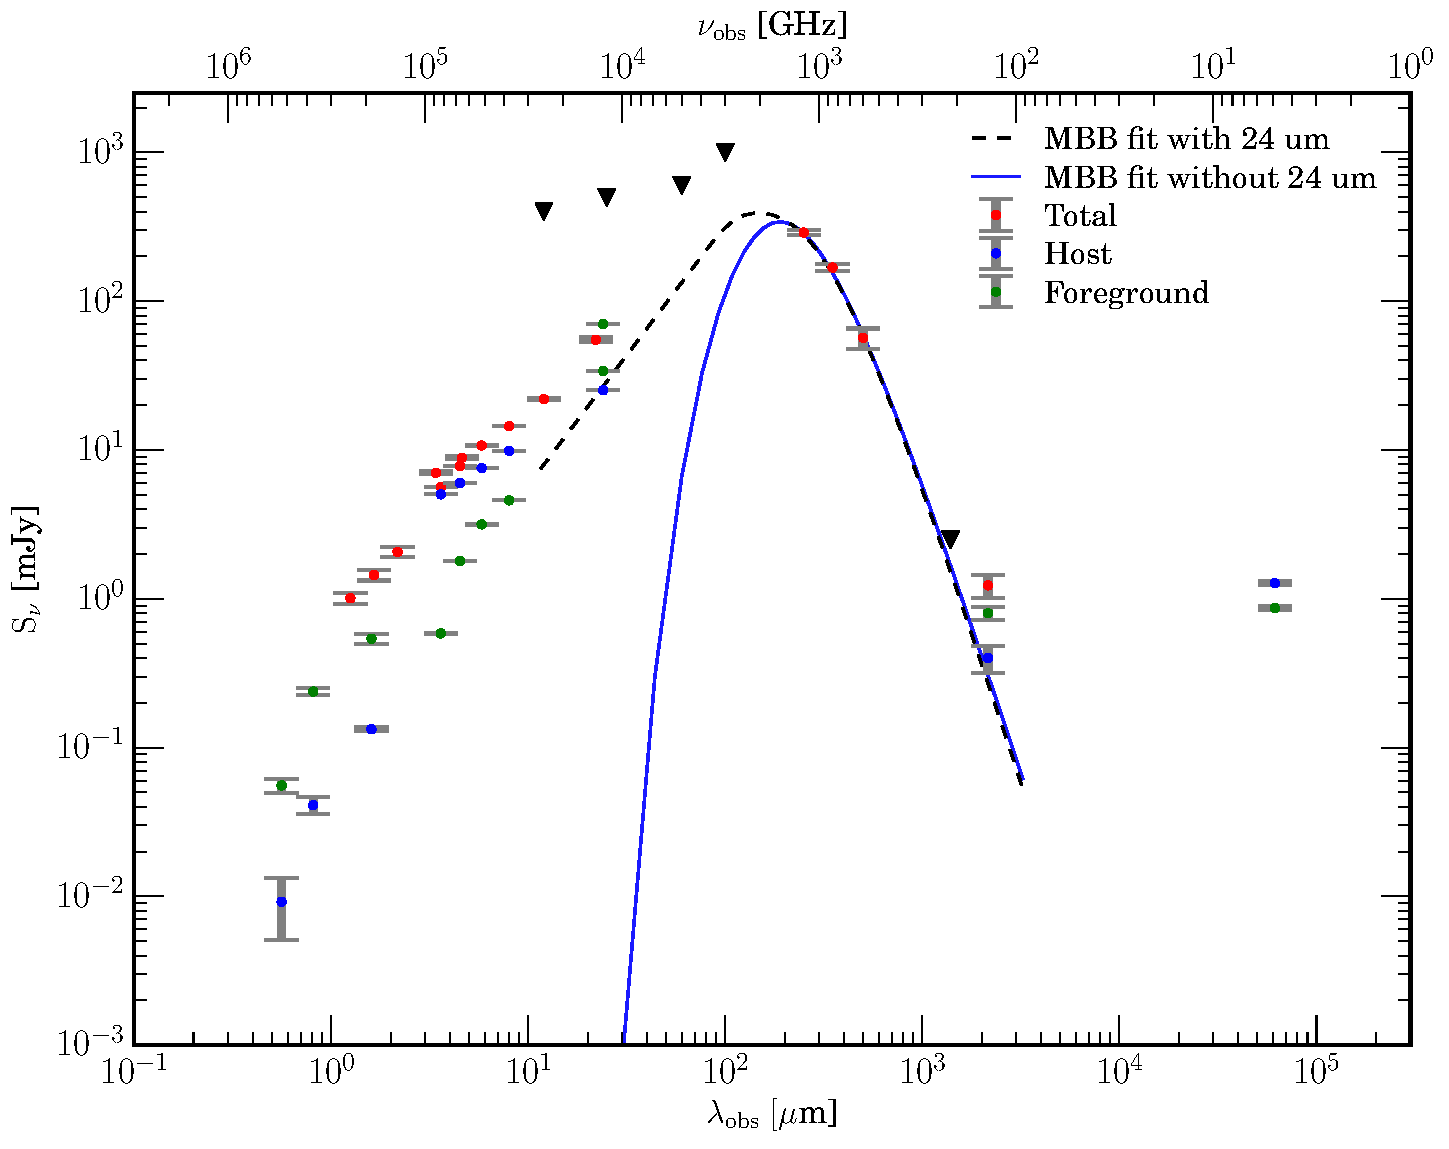
\includegraphics[trim=5 5 5 5, clip, width=0.45\textwidth]{../Figures/FullSED}
\caption{SEDs of RXJ1131 and its lensing galaxy. The photometry is listed in \Tab{photometry}.
Best-fit SED models of the thermal dust emission towards RXJ1131
with(out) MIR constraint at 24\,$\micron$ are plotted as dashed (solid) lines.
\label{fig:SED}}
\end{figure}

\subsection{ISM Properties} \label{sec:properties}
In this section, we derive the gas properties of the merging system
based on \bco and compare them with those reported by
C13 --- the largest sample of ULIRGs at similar redshift
(0.6\,$<$\,$z$\,$<$\,1.0) with CO measurements\footnote{The
\fir luminosity in C13 is derived based on 60\,$\micron$ and 100\,$\micron$ IRAS fluxes,
and using a different definition of
\LFIR: rest-frame 40\,$-$\,500\,\micron. Following this convention,
we find a \fir luminosity of
\LFIR = $($8.8\pmm0.4$)$\E{11}$(\mu_{\rm L}$/5.5$)\pmOne$\,\Lsun and
a SFR of $($150\pmm70$)$\,\sfrU for RXJ1131.}.
Their results are based on unresolved \bco and \rot{4}{3} line observations with the
IRAM 30-m single-dish telescope.

\subsubsection{Linewidth and Sizes} \label{sec:sizes}
A FWHM linewidth of $\Delta v_{\rm}$\,$\sim$\,600\pmm160\,\kms found
for RXJ1131 by fitting a single Gaussian
is considerably larger that those in the \citetalias{Combes13a} sample
(370\,\kms) as well as in
local ULIRGs \citep[300\pmm85\,\kms, with the largest being 480\,\kms;][hereafter S97]{Solomon97a}.
%ULIRGs (z < 0.3) studied in CO(1-0) by Solomon97a: ~1/3 of them have double-peaked or flat-topped spectrum. But their linewidths are based on single Gauss fit.
Yet, given the dynamic nature of these galaxies,
a CO linewidth of $\sim$600\,\kms may not be surprising.
Indeed, a linewidth of $\Delta v$ = 750\,\kms has been observed
in a local LIRG \citep[Arp 118; ][hereafter SV05]{SV05a}.
Linewidth of this range ($\gtrsim$500\,\kms) is also commonly observed in 
high-$z$ starburst galaxies  \citep[\eg][hereafter G05]{Greve05a} 
% \citep[780\pmm320\,\kms; \eg][hereafter G05]{Greve05a} 
and high-$z$ quasar host galaxies \citep[\eg][]{Coppin08a},
% \citep[550\pmm180\,\kms; \eg][]{Coppin08a}, 
which are 
believed to originate from mergers.
\defcitealias{Solomon97a}{S97}\defcitealias{Greve05a}{G05}\defcitealias{SV05a}{SV05}

The CO gas in RXJ1131 is $\sim$6\pmm3\,kpc in radius (in the source plane),
which is more
extended than the average in a sample of disk-like U/LIRGs studied by
\citet[]{Ueda14a}, % who find an average radius of 3.5\pmm2.3\,kpc 
but consistent with their range of 1.1\,$-$\,9.3\,kpc.
Our CO size is also consistent with that of high-$z$ 
($z$\,$>$\,1) galaxies \citep[$R\sim$\,4$-$20\,kpc;
\citetalias{Greve05a};][]{Daddi10a, Riechers11a, Ivison11a} and
local U/LIRGs in the \citet{Gao99a} sample ($R\lesssim$10\,kpc).
%For instance, extended molecular disks are often associated with advanced mergers
%\citep[\citetalias{Downes98a};][]{Gao99a}.but see also U14 for outliers
% with extended molecular gas in merger remnants

\subsubsection{Dynamical Mass}
Assuming the gas is virialized,
the dynamical mass can be approximate as
$M_{\rm dyn} = \sigma^2 R / G$,
where $\sigma$ is the velocity dispersion, or the rotational velocity in the case of a rotating disk model
$($\ie $\sigma$ = $V_{\rm rot}\, \sin\, i)$.
Using a rotational velocity $V_{\rm rot} \, \sin\, i$\,=\,345\,\kms (see \Sec{dynamics}),  % uncorrected for inclination
we find a dynamical mass of
$M_{\rm dyn}$\,$\sin^2 i$\,$(<$\,6\,kpc$)$ = 17\E{10}\,\Msun enclosed
within the CO-emitting region in RXJ1131.
If we instead consider the
\bco line peak separation $(\Delta v_{\rm sep}/2 \sim$200\,\kms$)$ as the rotation velocity, we find
$M_{\rm dyn}$\,$\sin^2 i$\,$(<$\,6\,kpc$)$ = 5.8\E{10}\,\Msun.
We derive an inclination angle of 56.4$\degr$ from the
morphological axial ratio of $a/b\sim$1\farcs8$/$3\farcs25, which we estimate
from the source-plane image reconstructed by \citetalias{Claeskens06a} (Figure 3 in their paper).  
This corresponds to an inclination-corrected dynamical mass of
8.3\E{10}\Msun$<$\,$M_{\rm dyn}$\,$<$\,25\E{10}\Msun.
Our estimate should be considered at best an upper limit since
the gas in RXJ1131 is unlikely virialized.
In the following sections, we use the
lower limit (8.3\pmm1.9)\E{10}\,\Msun as the dynamical mass as it is
derived in a manner similar to what is commonly used in literature 
(\eg \citetalias{Solomon97a}; \citealt[hereafter DS98]{Downes98a}; \citetalias{Greve05a}).
\defcitealias{Downes98a}{DS98}

Using the velocity dispersion obtained by fitting a single Gaussian to the
line profile of the companion ($\sigma$ = 30\,\kms)
and its intrinsic source size of $\sim$700\,pc obtained from the {\em HST}
$V$-band lens model \citepalias{Brewer08a},
we find a dynamical mass of $M_{\rm dyn}$\,$\sin^2 i$ = 5\E{6}\,\Msun.
This corresponds to $M_{\rm dyn}$\,=\,2\E{7}\,\Msun if we assume an
inclination angle of 30$\degr$.
We adopt the $V$-band size as the radius $R$ in the above estimate 
owing to the fact that it is the least uncertain source size constraint available for the companion.
However, since this dynamical mass is substantially lower than the gas mass, which is 
a more reliable estimate based on the data in hand, 
we do not use this dynamical mass to derive other physical parameters.
The inconsistency between the gas mass of the companion and its dynamical mass
may indicate its dusty nature, which causes the $V$-band source size to 
appear much smaller than its true extent without any dust obscuration.
% On the other hand, we find a half-right radius of $R_{\rm CO}$\,=\,4.2\pmm2.8\,kpc from our lens 
% model, which can only serve as a crude measure of its unobscured source size (see \Sec{caveat}). Using this CO size, we find a dynamical mass of $M_{\rm dyn}$\,=\,3\E{7}\,\Msun. WHICH is STILL LOWER THAN the GAS MASS?

%%% using disk model, should use FWHM of single Gauss fit then (Fu+13)
%Using $M_{\rm dyn}$\,$\sin^2 i$ = 4\E{4}\,$v_{\rm FWHM}^2\,R$
% \citep{Neri03a}, which assumes a disk geometry,  and our estimate of $V_{\rm rot}$ as
%$v_{\rm FWHM}$, we find a dynamical mass of
%$M_{\rm dyn}$\,$\sin^2 i$\,$(<$\,6\,kpc$)$ = 3\E{10}\,\Msun enclosed
%within the CO-emitting region.
%If we instead consider the
%\bco line peak separation $(\Delta v_{\rm sep}/2 \sim$200\,\kms$)$ as the rotation velocity, we find
%$M_{\rm dyn}$\,$\sin^2 i$\,$(<$\,6\,kpc$)$ = 1\E{10}\,\Msun.
%To correct for the inclination effect, we
%infer an inclination angle of 56.4$\degr$ using
%the morphological axial ratio ($a/b\sim$1\farcs8 / 3\farcs25)
%from the reconstructed image (Figure~3 in \citetalias{Claeskens06a}). This inclination angle
%is consistent with the
%observed unobscured AGN and an observable double peak line profile.
%The dynamical mass is then
%1.4\E{10}\Msun\,$<$\,$M_{\rm dyn}$($<$6\,kpc)\,$<$\,4.3\E{10}\Msun.
%% the systematic uncertainty on the inclination angle may cause this estimate to differ by
%% a factor of $\sim$2.
%Our estimate is likely a lower limit given the presence of a companion. In a merger model,
%the dynamical mass would be a factor of $\sim$2 higher \citep[and references therein]{Neri03a}.

\subsubsection{Gas Mass and Gas Ratios}
%%%%%%%%%%%%%%%%%%%%%%%%%%%%%%%%
% gas to dust ratio:
%%%%%%%%%%%%%%%%%%%%%%%%%%%%%%%%
% Solomon+97: GDR ~ 100
% single disk: 90 (converted conversion factor to 0.8) (Sanders91a)
% our galaxy MW ~150 (Draine+07)
% 120 (Li & Draine 2001) to ?160 (Zubko et al. 2004) to ?180 (Draine et al. 2007, and references therein)
% Wilson+08: U/LIRGs: abstract: 120+/-28 (rms deviation 109) in the most central kpc; paper content: 215+/-53 (rms 207); but 50-70 for ULIRGs only
%
% %%%%%%%%%%%%%%%%%%%%%%%%%%%%%%%%%%
Using the lensing-corrected dust mass, we find a galactic-scale gas-to-dust ratio of
40\pmm34, which is lower than the statistical average of $f_{\rm gas-dust}$\,=\,206
in the \citetalias{Combes13a} sample but well within their broad 
range of values over the entire sample. Our ratio is also consistent with 
high-$z$ SMGs 
% \citep[78\pmm26;][]{Bothwell13a} 
\citep[hereafter B13]{Bothwell13a} and
local ULIRGs \citep{Wilson08a}, but lower than of the Milky Way by
$\sim 4\sigma$ \citep[ignoring systematic uncertainties;][]{Li01a,Zubko04a,Draine07a}.
We note that the dust mass derived for RXJ1131 is poorly constrained.
If we adopt a dust mass from the other SED fit (\ie without constraints at 24\,$\micron$),
the dust mass is reduced by a factor of $\sim$2. \defcitealias{Bothwell13a}{B13}

There are a number of systematic uncertainties associated with this quantity. For instance,
the mass opacity coefficient $\kappa$,
the \alphaco conversion factor, and the brightness temperature ratio $r_{\rm 21}$.
If we instead use the ``Galactic'' \alphaco value, which may be more appropriate for some ULIRGs \citep[\eg][]{Papadopoulos12a} and minor mergers \citep{Narayanan12a},
the gas mass (and thus gas-to-dust ratio) would be $\sim$6 times higher.
We note that this gas mass is physically feasible based on dynamical mass constraint. 
On the other hand, we would also obtain a higher gas mass if
we assumed sub-thermal excitation between \bco and \aco emission, but
we expect this to be a minor effect as CO emission in ULIRGs are thermalized up to $J$ = 3 or 4.
We also note that the gas-to-dust ratio derived for RXJ1131 maybe biased low as the gas is likely to
be more extended than the dust. Consequently, the overall magnification factor 
for the CO gas may be lower than the optically thick dust, which dominates the \fir
luminosity, and thus leading to an overestimated dust mass 
via our adoption of the CO magnification factor. 

\subsubsection{SFE and Depletion Timescales}
% SFE:
% in terms of LFIR/Mgas:
% high-z: $>$100
% Greve+05: 450 +/- 170 Lsun/Msun for SMG
% Solomon97a: 180 +/- 160 Lsun/Msun
% SV05: local (z<0.1 spirals) of SFE < 100

% in terms of LFIR/L'CO:
% Greve+05: SMG 360 +/- 140 Lsun (K km/s pc^2)^-1
% Solomon97a: LFIR/L'CO = 160

To first order, the star formation efficiency
$($SFE = \LFIR$/$$M_{\rm gas})$ indicates the \SF rate per unit solar mass of molecular gas available in a galaxy.
Using a wavelength range of 40\,$-$\,500\,$\micron$ defined
in \citetalias{Combes13a} as the far-IR luminosity,
we find an SFE of 58\pmm10 \Lsun $M_{\odot}^{-1}$,
which is on the low end among other U/LIRGs at $z$\,$<$\,0.6
% \citep[$\sim$180\pmm160 \Lsun $M_{\odot}^{-1}$;][]{Solomon97a, Combes11a}
\citep[\citetalias{Solomon97a};][]{Combes11a} but consistent with those of
low-$z$ spiral galaxies \citepalias[$z$\,$<$\,0.1;][]{SV05a} and high-$z$ disk-like galaxies \citep{Daddi08a}.
Assuming an \alphaco of 0.8\,\alphaU is appropriate for RXJ1131, this would imply that
it is converting gas into stars at an efficiency 
similar to those of ``normal'' star-forming
disk-like galaxies rather than starburst galaxies
\citep[][\citetalias{Combes13a}]{Tacconi08a, Riechers11a}. 
This is in agreement with its disk-like kinematic signatures.

Results from theoretical simulations have suggested that 
the disk component of a gas-rich progenitor galaxy can 
survive merging if it has a low star formation efficiency, which in turn
reduces the gravitational torque available to 
remove the angular momentum of the gas, thereby allowing
a higher gas fraction to be retained and redistributed over a large extent in
the merged galaxy \citep{Hopkins09a}. With this, it is plausible that RXJ1131 
will evolve into a disk galaxy with a small bulge component upon merging given its low SFE.
%since there is little/no significant stellar material % (collisionless)
%available to torque away the cold gas in the disc, thus little/no angular momentum is lost,
%and gas will rapidly reform a cold disc in the background
%of the relaxing stellar potential.
% --> suppress the formation of a bulge in mergers of gas-rich discs (even in major merger)
% the final product will have a low bulge mass fraction.
%
%i.e. small bulge disc can also form from minor merger or major merger (if gas fraction is sufficiently large).
% 1:1 gas-riich mergers can yield disc-dominated remnants, and 1:3-1:4 ratio major mergers can yield B/T < 0.2.

% Depletion time:
% Greve+05: ~40 Myr
Assuming the \SF continues at the current rate without gas replenishment, this corresponds to a 
gas depletion time of $\tau$\,=\,102\pmm25\,Myr.
Since the \SF rate is expected to vary in an interacting system and
AGN accretion also consumes some fraction of the gas, the depletion
timescale should only be considered as an upper limit. 
\defcitealias{Tacconi08a}{T08}


%====================================================================
%While the \alphaco conversion factor is commonly assumed to be 0.8\,\alphaU for
%for ULIRGs/starbursts, its numerical value depends on the ISM environment
% \citep[\eg][]{Narayanan11a}.
% For instance, it could be different in a
% dynamically turbulent galaxy, where the gas is warmer, more excited,
% and denser, than in a quiescent galaxy.
% In addition, the physical basis for deriving the gas mass from the CO luminosity is
% by assuming the ISM only consists of virialized, non-overlapping gas clouds,
% which is often not true in ULIRGs \citep[][\citetalias{Solomon97, Downes98a}]{Downes93a}.
% % the CO emitting gas in the centers of ULIRGs is unlikely to be virialized, but instead bound by the potential of the galaxy or from molecular gas in pressure equilibrium rather than gravitational equilibrium.

% % DS98: lower alphaCO for objects with extended surface gas densities, where gas temperature and velocity dispersion are higher; Mgas derived from radiative transfer model instead of using standard conversion factor, which yields the \alphaco = 0.8 UNIT for local ULIRGs.
% % Also see Scoville+97

 %As discussed in Solomon \& Vanden
 %Bout (2005), low-$z$ studies of ULIRGs have led to the
 %suggestion that the conversion factor could be several times
 %smaller (Downes et al. 1993; Bryant \& Scoville 1999, DS98). This can
 %arise in ULIRGs if the gas is concentrated in the nuclear
 %regions (as a result of dissipative galaxy merging) and the
 %molecular emission linewidths can be broadened by the galactic
 %dynamics associated with the stellar mass, not just the self-gravitating
 %gas mass as in individual GMCs in which the
 %standard conversion factor was derived. In addition, the mean
 %gas temperature and density may be different in the ULIRG
 %nuclei as a result of the intense star formation activity and since AlphaCO
 %should vary as density and temperature e.g. (Dickman et al. 1986).
 % Also should be a continuous distribution instead of a bimodal value (Narayanan+12).
 % Yet, from numerical models, it is found that mergers have lower alphaCO than
 % disk galaxies, thus we can derive an upper limit on the gas mass in the RXJ1131 merger system using a disk alphaCO factor.
% In a minor merger, the rise in gas temperatures and velocity dispersions are not as extreme as in major mergers. Hence, the rise in velocity-integrated CO intensity is not as large, and the X-factor (and thus alphaco) does not decrease as much {Narayana11a}.

%\subsubsection{Comparison with High-$z$ SMGs and BzKs}
%At high redshifts ($z$\,$\gtrsim$\,1), SMGs are the irregular, turbulent
%star-bursting galaxies with elevated specific \SF rates (CITE) %\citep[sSFR][]{}
%and BzKs are the ``normal" star-forming disk galaxies with relatively lower
%\SF efficiencies, \SF rates and also
%longer depletion times \citep[\citetalias{Daddi10a};][]{CW13}.

%In fact, an \alphaco conversion factor of 3.6\pmm0.8
%has been proposed for BzKs using kinematic analysis/dynamical model (based on the dynamical mass; e.g. Daddi10a).
% Whereas \citet{Tacconi08a, Carilli10a} place an upper limit of $\sim$0.8 on high-$z$ SMGs, leading the emergence of two star formation modes. Carilli+10: based on dynamical constraints
%====================================================================

%--------------------------------------------------------------------------
%                                Discussion
%--------------------------------------------------------------------------
\section{Discussion} \label{sec:diss}
\subsection{Fate of RXJ1131-1231}
The classical picture for mergers is one where they are responsible for the formation of the local
red and passive spheroidal galaxies.
With more realistic treatments of star formation and feedback in recent simulations,
it has been suggested that it is possible to suppress bulge formation
in gas-rich mergers, thereby forming large disks 
that resemble local spiral galaxies \citep{Springel05a, Robertson06a, Hopkins09a}.
% (bulge dominated; Springel05a, Robertson06a)
% and disc with low B/D ratio ($\sim$0.1$-$0.2; Hopkins09a).
%
%In systems that are sufficiently gas-rich, it is possible to
%suppress the formation of a bulge in mergers of gas-rich discs (even in major merger)
%since there is little/no significant stellar material % (collisionless)
%available to torque away the cold gas in the disc, thus little/no angular momentum is lost,
%and gas will rapidly reform a cold disc in the background
%of the relaxing stellar potential.
%Gas, being collisional, cannot violently relax, but must
%have its angular momentum torqued away in order to dissipate and
%build a bulge by forming stars in a central starburst
%(\ie gas loses angular momentum to stars in the
%perturbed disk and fall toward center).
% In a merger,
%this torque is primarily internal, from stars in the same disc: the
%passages and merger of the secondary induce a non-axisymmetric
%distortion in the primary stellar and gas disc. The stellar distortion
%(in a trailing resonance and close proximity to the gas response)
%efficiently removes angular momentum from the gas and allows it
%to fall to the center and form a bulge  (see also Barnes \& Hernquist
% 1996).
% A bulge will form because cold gas with no angular momentum
% will be largely unable to form any sort of disk, and that a galaxy?s
% worth of gas compressed to high densities and small
% radii will inevitably form a large mass in stars).
%
% unlikely RXJ1131 will evolve into present-day massive
% ellipticals (M$\gtrsim$1\E{12}\,\Msun),
% gas-poor mergers: --> present-day massive elliticals
% (Boylan-Kolchin, Ma & Quataert 2005, 2006; Naab, Khochfar & Burkert 2006; Robertson B., Cox T. J., Hernquist L., Franx M., Hopkins P., Martini P., Springel V., 2006a, ApJ, 641, 21; Cox et al. 2006b)
The extended molecular gas distribution in RXJ1131 together with its low SFE implies that the 
removal of angular momentum of the gas via gravitational torque is inefficient.
Other mechanisms e.g. bar-like structures that are more efficient at removing angular momentum will 
be required in order to transform the gas disk of RXJ1131 into a stellar spheroid and evolve into 
an E/S0 galaxy. Without these, it is more conceivable that RXJ1131 will retain its disk component and
evolve into a disk galaxy upon its final coalescence with the companion.

\subsection{Velocity Offset and a Recoiling Black Hole}
Using the CO line center redshift as the systemic redshift, we find
a velocity offset of $\sim$780\,\kms from the optical
\mgii line and the \oiii lines \citepalias[$z_{\rm QSO} = 0.658$;][]{Sluse03a}. This implies that the AGN is dynamically offset from the centroid of its host galaxy. 
From the CO channel maps in \Fig{CO21mom} and \Fig{chanmap}, it is also apparent that the 
line center of the gas is not co-spatial with the optical quasar as the point-like images
along the lensing arc
are spatially offset to the NW of the CO line center.
While spatial offsets between optical lines and CO line
have been reported in other galaxies, the velocity offsets are typically $\lesssim$\,500\kms.
{\bf
In the classical SDSS analysis for line offsets \citep{Richards02a}?.
\oiii and \mgii analysis \citep{Boroson05a, Bae14a}?.
with the corresponding trends and possible explanations?.
More extreme offsets between CO and optical lines have been seen \citep{Hainline04a} 
or between \cii and \mgii \citep[\eg][]{Venemans16a}.}
For instance, the
velocity offset in
an SDSS sample of ongoing mergers at $z$\,$<$\,0.21 is at most $\sim$410\,km/s \citep{Comerford14a}.

A large velocity offset can also result from a recoiling black hole (BH) where its broad line region
is moving at high velocity relative to the bulk of its host galaxy 
\citep{Madau04a, Bonning07a, Loeb07a}. 
Such a scenario is expected to occur 
when a pair of uneven mass BH coalesce, during which their orbital energy is being released 
as gravitational wave and a 
non-zero net angular momentum is being carried away.
Depending on their initial conditions, numerical relativity simulations have shown that
the recoil velocity can reach up to $\sim$4000\,\kms for spinning BHs \citep[\eg][]{Campanelli07a}.
%While such large velocity offsets are theoretically achievable,
%they are not commonly observed --- only a few objects 
%have been reported with optical offsets $\gtrsim$1000\,\kms. For instance,
%the most promising candidate with both spectroscopy and imaging
%signatures of a recoiling BH is CID-42 at $z$\,=\,0.359, with 
%an offset of $\sim$1300\,\kms between the narrow and broad component of H$\beta$ \citep{Civano10a}.
%Other example includes the type-1 QSO SDSS 0956+5127 at $z$\,$\sim$\,0.714, with an offset of 1200\,\kms
%between Mg{\scriptsize II}~2798\AA\ and $[$O{\scriptsize III}$]$~4959, 5007\AA\ lines
%\citep{Steinhardt12a}. % but here its between CO and optical lines
%% SDSSJ0927+2943 at $z$\,$\sim$\,0.713, with an offset of 2650\,\kms \citep{Komossa08a}, but disproved by Decarli+14; Hence, I am going to cut this out because I listed this source here just to demonstrate the scarcity of high velocity offsets; but the offset in this system is between a set of redshifted versus a set of blueshifted.. which is not quite the same our case here.
The fact that the BH in RXJ1131 has a high spin parameter \citep{Reis14a}
renders this scenario a viable option for the origin
of the velocity offset. 
However, since this model requires a merged BH, this interpretation would imply RXJ1131 have 
already encountered with the companion galaxy, which is consistent with
the highly spinning BH observed in RX1131.
Given the presence of a nearby companion observed in our data, the system may be in its 
subsequent stages of (minor) merging resulting from previous passage of a major merger.

As demonstrated here using \mgii and \oiii lines, large velocity offsets between CO and optical lines may be present.
We thus caution against the use of optical lines as 
true systematic redshift indicators as the resulting redshift can deviate from the 
true value.

\subsection{The \bhrelation Relation}


Comparing the spatial extents of the CO with the stellar components traced by {\it HST}\\
The dusty nature of this system?? \\

\citet{Shields06a} investigate the \bhrelation relation to high-$z$ using CO line width since 
CO has been detected in over hundreds of galaxies at $z$$>$1.
From their results, the dynamical mass from CO line widths is 
smaller than would be expected by the local relation, but they also noted it is possible that the stellar dispersion is
underestimated (see section 2.3 in Shields06a).


If we follow their approach, and use the CO linewidth to derive $\sigma_*$, assuming FWZI = 2$v_\textrm{rot}$, then the stellar dispersion is related to the CO dispersion via 
$\sigma_*$ = 4.44$\sigma_{\rm CO}$.
% FWHM ~ 2/3 FWZI; FWZI = 2*v_cir = 2sqrt(2) * sigma_*;  => FWHM ~ 0.53 sigma_*.
% where CO dispersion = FWHM/2.355 ---> sigma_* = 4.44 * CO dispersion.
, we find?.

If we adopt the broad H$\beta$ line as a proxy to the black hole mass using the virial method/estimator, then we find \mbh = 6\E{7}$-$1.3\E{8}\,\Msun \citep{Peng06a, Dai10a}, depending on the normalization. 

%see Coppin08
%see section 5.2 in Bothwell13a
%
{\bf compare to J04135 in R13} \\


%--------------------------------------------------------------------------
%                                Conclusions
%--------------------------------------------------------------------------
\section{Summary and Conclusions} \label{sec:sum}
% see Hodge12_dynamics.pdf for guide

We observe \bco and \cco line emisison toward the
quadruply-lensed quasar RXJ1131 at $z_{\rm CO}$\,$\sim$0.65 
using the PdBI and CARMA, benchmarking the 
first resolved interferometric CO imaging at intermediate redshift.
The brightness temperature ratio between \bco and \cco of $r_{32}$ = BLAH, which taking into 
account the large phase errors associated with \cco, is consistent with
thermalized excitation between these lines in other ULIRGs.
The (gas) mass ratio, the intrinsic CO line profile,
and the source-plane velocity field are all evident of
a minor merger, in good agreement with previous studies of RXJ1131 in the optical \citepalias{Claeskens06a,Brewer08a}. 

% explicit discussion of RXJ1131 being IR luminous, and gas-rich
Our analysis of the cold gas kinematics and dynamics of RXJ1131 find 
characteristics resembling a rotating disk. 
The intrinsically symmetric double-horned line profile, the smooth and
symmetric velocity field/gradient seen in both the source plane from our lens model as well
as in the image plane, consistent with the findings from previous optical lens model 
suggesting a kinematically-order rotating disk galaxy.
The high dispersion $\gtrsim$400\,\kms near the dynamical center also
suggest that RXJ1131 is turbulent, albeit lack of spatial resolution. 
Our results confirms the presence of the optically faint companion with CO detection
suggested by previous studies. 
Assuming same CO excitation, we find a gas mass of BLAH in
the companion. Using the gas mass ratio of ($\sim$7:1)between RXJ1131 and the companion, this 
implies the system is a wet minor merger.
We thus conclude that RXJ1131 is a ULIRG hosting a massive gas reservoir in a disturbed/turbulent
disk, undergoing merging with a nearby companion (aka a wet minor merger).

The SFE is similar to that nearby spiral galaxies and high-$z$ disk-like galaxies rather than 
ULIRGs or high-$z$ starbursts galaxies at $z$$\gtrsim$0.6. Implying BLAH
Our result is consistent with the emerging consensus on
the correlation between molecular gas content and redshift,
suggesting it as the explanation for the elevated SFR at high redshift/
the observed trend in the cosmic SFH.
Given our large error bar on the gas mass fraction, we cannot constrain its evolution 
but our result is consistent with a decreasing trend of gas fraction
since $z$\,$\approx$\,1.0 \citep{Combes13a}; but is consistent with 
in both ULIRGs samples in redshift bins of 0.2\,$<$\,$z$\,$<$\,0.4 and 0.6\,$<$\,$z$\,$<$\,1.0 within the uncertainties.

The compact UV emission, which can be a starburst resulting from gas accumulation
owing to a non-axisymmetric perturbation from the companion.
% the stellar component torques away the angular momentum, allowing the gas to fall inward.
Dusty nature of companion?
The IR luminosity also agrees with the results from previous low-$z$ studies: AGNs are
typically found in late stage mergers \citep{Yuan10a,Iwasawa11a,Carpineti12a} and
only major mergers near their final coalescence can provide \LIR$>$\,10$^{12}$\,\Lsun,
\citep[\eg][]{Carpineti15a,Larson16a}. In contrast to the 
galaxies with ULIRG-like IR luminosity high-$z$, are believed to be in some stages of merging.

The highly spinning black hole in RXJ1131 is also consistent with
this hypothesis.
If we favor the gravitational wave recoil mechanism
to explain the optical velocity offset, it would also imply the black
holes (and their host galaxies) have merged or are at their final coalescence.

The optical lines are at a velocity offset of $\sim$780\,\kms from the systematic redshift is consistent 
with possible black hole recoil. 
Given the BLAH, it is plausible that RXJ1131 is in its late stage of merging and 
possibly encountered with its companion previously, consistent with 
compact SB traced by $V$-band image triggered by gas inflow/accumulation toward nuclear regions 
arising from perturbations in the disk from/interactions with the companion.
%Our results indicate a self-consistent picture of ... followed by gravitationally instability and SF in a massive, gas-rich disk and a subsequent build-up of a central bulge through inflow triggered by disk installbilities and/or minor merger.
Theoretical simulations suggest disk in progenitor galaxy may be retained post-merging in gas-rich 
mergers. BLAH. Thus, the merging system studied here will likely evolve into a merged disk galaxy.

% broader
Gas-rich major mergers are commonly likely the origins of high-$z$ quasar host galaxies as
they are frequently observed with companions and from theoretical point of view. But considerate 
interest in understanding the mechanisms in turning off \SF and AGN accretion since $z$$\sim$2, as 
encoded in the \bhrelation. Thus, studies of galaxies at intermediate redshifts are crucial to 
bridge the connection between local relation and high-$z$. 
The study of this relation is hampered at intermediate redshift due to the difficulties in observing the 
stellar emission in the host galaxy from the much brighter quasar. 
The use of dynamical mass as a proxy to the \bhrelation have been proposed in a few high-$z$ studies 
but requires resolved observations to provide constraints on the spatial extent tracing the potential of 
the host galaxy. Lensing likely the the way to allow observations of quasar emission and 
host galaxy emission. Dynamical lens modeling provides a promising avenue to study the velocity 
structure and dynamics of the cold gas in greater detail. 
To date, only a few other studies using similar techniques \eg other luminous,
gas-rich interacting galaxies and mergers.
This study of RXJ1131 serves as a benchmark/demonstrate the use of gravitational lensing and 
dynamical lens modeling for further high-resolution molecular gas studies at 
intermediate redshifts.  Similar resolved CO studies are needed to investigate the evolution in 
the $M_{\rm BH}$$-$$M_{\rm dyn}$ relation to understand the co-evolution of SMBHs and their 
host galaxies through cosmic time.

%==============================================================================
%                                Back matters
%==============================================================================
% ACKNOWLEDGEMENTS
%-----------------
\acknowledgments
This work is based on observations carried out under project number S14BX
with the IRAM NOEMA Interferometer. IRAM is supported by INSU/CNRS (France), MPG (Germany) and IGN (Spain).
Support for CARMA construction was derived from the Gordon and Betty Moore
Foundation, the Kenneth T. and Eileen L. Norris Foundation, the James S.
McDonnell Foundation, the Associates of the California Institute of
Technology, the University of Chicago, the states of Illinois, California, and
Maryland, and the National Science Foundation. Ongoing CARMA development and
operations are supported by the National Science Foundation under a
cooperative agreement and by the CARMA consortium universities.
The National Radio Astronomy Observatory is a facility of the National Science
Foundation operated under cooperative agreement by Associated
Universities, Inc.
This research made use of data obtained with {\it Herschel}, an ESA space
observatory with science instruments provided by European-led Principal
Investigator consortia and with important participation from NASA.
This research has made use of NASA's Astrophysics Data System Bibliographic
Services.
This work is based in part on observations made with the \spitzer,
which is operated by the Jet Propulsion Laboratory, California Institute of
Technology under a contract with NASA.
This publication made use of data products from the Wide-field Infrared
Survey Explorer, which is a joint project of the University of California, Los
Angeles, and the Jet Propulsion Laboratory/California Institute of Technology,
funded by the National Aeronautics and Space Administration.
This publication made use of data products from the Two Micron All Sky
Survey, which is a joint project of the University of Massachusetts and the
Infrared Processing and Analysis Center/California Institute of Technology,
funded by the National Aeronautics and Space Administration and the National
Science Foundation.
This research made use of the NASA/IPAC Extragalactic Database (NED) which
is operated by the Jet Propulsion Laboratory, California Institute of
Technology, under contract with the National Aeronautics and Space
Administration.
This research made use of Astropy, a community-developed core Python package for Astronomy \citep{astropy}.
This research made use of APLpy, an open-source plotting package for Python hosted at \url{http://aplpy.github.com}.

Facilities: IRAM PdBI, CARMA, VLA, Herschel(SPIRE), WISE, IRAS, 2MASS, Spitzer(IRAC, MIPS), HST(ACS, NICMOS)


  %--------------------------------------------------------------------------
  %                               Bibliography
  %--------------------------------------------------------------------------
\bibliographystyle{yahapj}
\bibliography{RXJ.bib}
\end{document}